\documentclass[hidelinks,12pt,a4paper]{book}
\usepackage{hyperref}
\usepackage{geometry}\geometry{top=5cm,bottom=2cm,left=3cm,right=3cm}
\usepackage{amssymb}
\usepackage{amsmath}
\usepackage{amsthm}
\usepackage{lmodern}
%\usepackage{mathtools}
%\usepackage{commath}
\usepackage{algorithm}
\usepackage{algorithmic}
\floatname{algorithm}{Algoritmo}
\renewcommand{\listalgorithmname}{Lista de algoritmos}
\renewcommand{\algorithmicrequire}{\textbf{Entrada:}}
\renewcommand{\algorithmicensure}{\textbf{Salida:}}
\renewcommand{\algorithmicend}{\textbf{fin}}
\renewcommand{\algorithmicif}{\textbf{si}}
\renewcommand{\algorithmicthen}{\textbf{entonces}}
\renewcommand{\algorithmicelse}{\textbf{si no}}
\renewcommand{\algorithmicelsif}{\algorithmicelse,\ \algorithmicif}
\renewcommand{\algorithmicendif}{\algorithmicend\ \algorithmicif}
\renewcommand{\algorithmicfor}{\textbf{para}}
\renewcommand{\algorithmicforall}{\textbf{para todo}}
\renewcommand{\algorithmicdo}{\textbf{hacer}}
\renewcommand{\algorithmicendfor}{\algorithmicend\ \algorithmicfor}
\renewcommand{\algorithmicwhile}{\textbf{mientras}}
\renewcommand{\algorithmicendwhile}{\algorithmicend\ \algorithmicwhile}
\renewcommand{\algorithmicloop}{\textbf{repetir}}
\renewcommand{\algorithmicendloop}{\algorithmicend\ \algorithmicloop}
\renewcommand{\algorithmicrepeat}{\textbf{repetir}}
\renewcommand{\algorithmicuntil}{\textbf{hasta que}}
\renewcommand{\algorithmicprint}{\textbf{imprimir}} 
\renewcommand{\algorithmicreturn}{\textbf{devolver}} 
\renewcommand{\algorithmictrue}{\textbf{cierto }} 
\renewcommand{\algorithmicfalse}{\textbf{falso }} 

\usepackage{graphicx}
\usepackage{subcaption}
\usepackage[spanish,es-lcroman]{babel}
\selectlanguage{spanish} 
\usepackage{ucs}
\usepackage[utf8x]{inputenc} %Codificación de entrada
\usepackage[T1]{fontenc} %Codificación de fuente
\usepackage{multirow}
\usepackage[nottoc]{tocbibind} %para que aparezca la biblio en el indice

\usepackage[usenames]{color}
\usepackage[dvipsnames]{xcolor}

\providecommand{\abs}[1]{\lvert#1\rvert}
\providecommand{\norm}[1]{\lVert#1\rVert}
\providecommand{\absbig}[1]{\lvert#1\rvert}
\providecommand{\normbig}[1]{$\left\|#1\right\|$}
\providecommand{\prodint}[1]{\langle#1\rangle}

\theoremstyle{plain}
%\newtheorem{thm}{Theorem}[chapter] % reset theorem numbering for each chapter
%\newtheorem{lemma}[theorem]{Lema}
\newtheorem{theorem}{Teorema}[chapter]
\newtheorem{corollary}{Corolario}[theorem]
\newtheorem{lemma}[theorem]{Lema}
\renewcommand\qedsymbol{$\blacksquare$}
\theoremstyle{definition}
\newtheorem{definicion}[theorem]{Definición} % definition 

\newtheorem{ejemplo}{{\textbf{Ejemplo}}}[chapter]
%\newcounter{ejemplo}[chapter]
%\newenvironment{ejemplo}{\refstepcounter{example}\noindent \textbf{Ejemplo}}{\hfill$\square$\\}

\decimalpoint
\setlength{\parindent}{10pt}
\raggedbottom

\renewcommand{\labelitemi}{$\bullet$}
\newcommand{\cmt}[1]{{\color{red}\fbox{#1}}}

\begin{document}

%----------------------------------------------------------------------------------------
%   PORTADA
%---------------------------------------------------------------------------------------
\thispagestyle{empty}

\begin{titlepage}
\begin {center}


\includegraphics[scale=.3]{uba2.jpg}

\medskip
\textbf{UNIVERSIDAD DE BUENOS AIRES}

\smallskip

\textbf{Facultad de Ciencias Exactas y Naturales}

\smallskip

\textbf{Departamento de Matemática}

\vspace{3.5cm}

\textbf{\large Tesis de Licenciatura}

\vspace{1.5cm}
\textbf{\large Sistemas de Recomendación: \\
Las máquinas de factorización y una aplicación al problema de arranque en frío}
\vspace{1.5cm}

\textbf{Gastón Elián Bujía}

\end {center}

\vspace{1.5cm}

\noindent \textbf{Director:} Leandro Lombardi

\vspace{3cm}

\rightline{Marzo 2018}

\end{titlepage}

\pagenumbering{Roman}
\setcounter{page}{3}

%----------------------------------------------------------------------------------------
%   AGRADECIMIENTOS
%----------------------------------------------------------------------------------------

\chapter*{Agradecimientos}
%\markboth{AGRADECIMIENTOS23}{AGRADECIMIENTOS} % encabezado 
\setlength\parindent{1cm}
En primer lugar quiero agradecerle a Leandro, por su confianza y consejos que me brindo a lo largo de esta tesis y la paciencia que tuvo para ayudarme en todo lo necesite. Así también quiero agradecerles a los jurados por tomarse el tiempo de leer esta tesis y corregirla.

A Exactas por todas las oportunidades brindadas y grandes experiencias vividas a lo largo de estos años y los que estan por venir.

A todos mis compañeros de la carrera con los que comparti tanto tiempo de cursadas, estudio, charlas y debates.

A Luz y a Yamila, que 

A Lucho por sus consejos, siempre presente ya sea estudiando o saliendo a tomar algo.

A los pibes de ecuaciones, Juan, Juan Z, Pepe y Javi, por las noches de estudio con mucha cerveza y siempre algo a la parrilla.

A mis compañeros de docencia, en especial a Eugenio y a Flor, mis compañeros en el 2017, por todo el aguante en los tramos finales de la carrera.

A Mauricio y Dario, MAUDAGA, por su apoyo constante en los tiempos más adversos, por ser compañeros de aventuras y noches de cerveza. Sin ellos, todo el camino recorrido hubiese sido mucho más dificíl.

A Agostina, Natalia y Matias, por los excelentes momentos vividos durante todo este tiempo juntos en Tecnopolis, las largas charlas de política y de la vida.

A mis compañeros de Tecnopolis, sobretodo a Seba, Ema, Chris, Aye, Nacho, Nico, Axel, por darme siempre más ganas de trabajar en Tecnopolis.

A Camila, Yamila y Sol, por ayudarme a preocuparme menos por todo y sacar las mejores carcajadas, siempre haciendome el aguante con unos mates o unas cervezas.

A Lucas, por su amistad incondicional y su eterno aguante a lo largo de tanto tiempo.

A Facundo, Nicolas, Leandro, Damian y Sergio, por las juntadas espontáneas y los vicios compartidos.

A Luciana, por ser mi hermana, por acompañarme, por los momentos compartidos, por ser un apoyo siempre.

A Beto, Ale, Ara, Mica y Juan, por los mates de domingo, las juntadas nocturnas, los debates, las charlas, las películas, siempre haciéndome sentir uno más de la familia. 

A Nacho y Gabi, por las tardes en la empresa vendiendo humo y las posteriores salidas a Finisterre.

A mis abuelas Irma e Isabel, que aunque ya no estan conmigo, siempre me acompañaran.

A mi hermano Mariano, por su confianza y apoyo, por sentirme siempre acompañado en todo.

Por ultimo, a mis viejos, sosten total de todo lo que pude hacer en mi vida. Gracias por el amor y la paciencia que me ayudaron a alcanzar mis metas, sin su apoyo nada de esto hubiese sido posible. Gracias siempre.




%----------------------------------------------------------------------------------------
%   TABLA DE CONTENIDOS
%----------------------------------------------------------------------------------------

\tableofcontents

%----------------------------------------------------------------------------------------
%   TESIS
%----------------------------------------------------------------------------------------
\mainmatter %empieza la numeración de las páginas
\pagestyle{headings}

\chapter*{Introducción}

Los sistemas de recomendación se han vuelto muy populares en los últimos años debido a la gran cantidad de información que existe gracias a la web. Los mismos se encuentran ampliamente extendidos en los ámbitos de las tiendas online, sitios de música, películas, libros, artículos, inmuebles o hasta recomendaciones sociales. Estos sistemas, tratan de recomendar a los usuarios diferentes artículos según sus gustos o necesidades, valiéndose de técnicas propias del aprendizaje automático.

El objetivo de esta tesis es la de realizar una introducción al tema, enfocándonos en una rama particular conocida como filtros colaborativos y las problemáticas relacionadas al área. En el primer capitulo realizaremos un resumen de las definiciones mas importantes, describiremos los algoritmos de recomendación clásicos de los filtros colaborativos y analizaremos diferentes formas de evaluar su rendimiento.

En el segundo capítulo, introduciremos las máquinas de factorización y veremos como aplicarlas en el ámbito de recomendación, comparando su rendimiento con las técnicas clásicas.

En el tercer capítulo, nos centraremos en uno de los problemas más importantes de los filtros colaborativos, conocido como el problema del arranque en frío. Describiremos algunas técnicas para mitigar este problema, y propondremos un acercamiento diferente.

En los últimos dos capítulos, detallaremos las simulaciones y experimentos llevadas a cabo para comparar el rendimiento de las máquinas de factorización con el resto de las técnicas y veremos como se comporta nuestra propuesta para el escenario de arranque en frío.

%%%%%%%%%%%%%%%%%%%%%%%%%%%%%%%%%%%%%%%%%%%%%%%%%%%%%%%%%%%%%%%%
%%%%%%%%%%%%%%%%%%%%%%%%%%%%%%%%%%%%%%%%%%%%%%%%%%%%%%%%%%%%%%%%
\chapter{Sistemas de recomendación}

En este capitulo definiremos que es un sistema de recomendación y haremos particular hincapié en un tipo específico de sistema conocidos como \textit{filtros colaborativos}. Describiremos los principales conceptos y definiciones, su clasificación así como las métricas de evaluación relacionadas y las técnicas clásicas en el área.

\section{Preliminares}

Los sistemas de recomendación son técnicas y herramientas que se engloban dentro del aprendizaje automático y la teoría de la recuperación de información. Su objetivo principal es predecir la valoración de un usuario sobre un objeto y recomendar a un conjunto de usuarios uno o más elementos de una lista predeterminada que pueden resultar de su interés. Dichos elementos que llamaremos \textit{items}, suelen pertenecer a alguna categoría específica de objetos como ser películas, libros, música, papers, documentos, noticias, etc.\cite{agg}. Para desarrollar esta tarea, los sistemas de recomendación utilizarán la información existente sobre la interacción entre los usuarios y los items.

Para poder medir el interés de un usuario \textit{u} sobre un ítem \textit{j} llamaremos $r_{uj}$ al \textit{rating} o valoración que tiene dicho usuario sobre ese ítem. Los posibles ratings $r_{uj}\in \mathcal{R}$, donde $\mathcal{R}$ será el conjunto de ratings, por ejemplo $\mathcal{R}=\{1,2,3,4,5\}$ o puede ser un rating binario donde $\mathcal{R}=$\{"Me gusta", "No me gusta"\}, o incluso venir de forma implícita como cantidad de clicks hechos sobre un ítem o si se compró el ítem o no. 

\begin{definicion}
Sea $R \in \mathbb{R}^{n\times m}$ la matriz de ratings usuarios-items, donde las filas representan a los $n$ usuarios y las columnas a los $m$ items:

\[
R =
\begin{pmatrix}
r_{1 1} & r_{1 2} & \cdots & r_{1 m}\\
r_{2 1} & r_{2 2} & \cdots & r_{2 m}\\
\vdots & \vdots & \ddots & \vdots \\
r_{n 1} & r_{n 2} & \cdots & r_{n m}\\
\end{pmatrix}
\]

Las entradas $(u,j)$ representan el rating $r_{uj}$ del usuario $u$ sobre el ítem $j$. Los valores conocidos de la matriz $R$ los llamaremos $S$ y llamaremos el conjunto de índices de dichos valores como $\mathcal{K}=\{(u,j):r_{uj} \text{ es observado}\}$.
\end{definicion}

La matriz usuario-ítem $R$ del sistema de recomendación es una matriz con una gran cantidad de valores faltantes, esto se debe en general a la gran cantidad de items que suelen contar los sistemas de recomendación en comparación a los pocos que evalúan los usuarios, lo que representa una de las principales dificultades que enfrentan los sistemas. Por ejemplo, uno de los sistemas de recomendación mas conocidos es el brindado por la empresa Netflix, la cual ha contribuido significativamente al área con una competencia que se conoció como $The$ $Netflix$ $Prize$\cite{bennett2007netflix}. El conjunto de datos de entrenamiento para esta competencia contenía 100,480,507 clasificaciones que 480,189 usuarios dieron a 17,770 películas, con lo cual la densidad de la matriz de datos es aproximadamente $1.2\%$.

%%% Entorno ejemplo
\begin{ejemplo}
Supongamos que tenemos un sistema de recomendación de películas que utiliza un rating del 1 al 5, donde tenemos seis usuarios $U=\{u_1,\cdots, u_6\}$ y seis películas $I=\{i_1,\cdots, i_6\}$, y las evaluaciones observadas sobre las películas vistas vienen dadas por la matriz:

\begin{table}[htb]
\begin{center}
\begin{tabular}{|c|c|c|c|c|c|c|}
\hline
  & $i_1$ & $i_2$ & $i_3$ & $i_4$ & $i_5$ & $i_6$ \\
\hline
$u_1$  & 2 &  & 5 &  & 4 &  \\
\hline
$u_2$  &  & 3 & 1 &  &  & 4 \\
\hline
$u_3$  & 1 &  & 4 & 2 &  &  \\
\hline
$u_4$  &  &  & 3 &  & 5 & 3 \\
\hline
$u_5$  & 4 & 5 &  & 3 &  & 1 \\
\hline
$u_6$  &  & 2 &  & 4 & 4 &  \\
\hline
\end{tabular}
\end{center}
\end{table}
Los espacios en blanco representan las películas que no vieron los usuarios, por ejemplo el usuario $u_1$ vio la película $i_3$ y la evaluó con cinco puntos, entonces $r_{1,3} = 5$. Mientras que $u_1$ no vio las películas $i_2,i_4$ e $i_6$. \hfill$\square$
\end{ejemplo}


El objetivo principal de un sistema de recomendación, en este contexto, es predecir las entradas desconocidas de la matriz de rankings $R$, es decir la valoración $\hat{r}_{uj}$ del usuario $u$ sobre el ítem $j$, sin embargo pueden establecerse otros objetivos como hablaremos mas adelante. Para realizar dicha tarea hay varias estrategias en general que se pueden dividir en tres grandes categorías\cite{agg}:

\begin{description}
\item[Filtros Colaborativos] Los filtros colaborativos utilizan los ratings aportados por múltiples usuarios para poder estimar un rating desconocido de un ítem para un cierto usuario. Este tipo de técnicas son las mas estudiadas y utilizadas en los sistemas de recomendación. Describiremos este tipo de sistemas con mayor detalle mas adelante.
\item[Basados en Contenido] En los sistemas de recomendación basados en el contenido, los atributos descriptivos de los elementos se utilizan para hacer recomendaciones. El término $contenido$ se refiere a estas descripciones referidas a cualidades de los items. En los métodos basados en el contenido, las calificaciones y el comportamiento de compra de los usuarios se combinan con la información de contenido disponible en los artículos. Por ejemplo, supongamos que sabemos que un usuario valoró altamente una película dada, pero no conocemos el rating de otros usuarios respecto a esta película ni al usuario. Sin embargo, las características de la película pueden ser usadas para hacer una recomendación, en este caso el contenido que podríamos utilizar son el genero de la película, los actores, el director, el año de filmación, etc.
\item[Basados en Conocimiento] Los sistemas de recomendación basados en el conocimiento son particularmente útiles en el contexto de elementos que no se compran muy a menudo. Los ejemplos incluyen elementos tales como bienes inmuebles, automóviles, solicitudes de turismo, servicios financieros o bienes de lujo caros. En estos casos, como los artículos se compran raramente o simplemente el interés de un usuario sobre los mismos tiene mucha variabilidad en el tiempo, entonces no tenemos acceso a suficiente información para poder hacer una recomendación. Tales casos se pueden abordar con sistemas de recomendación basados en el conocimiento, en los que las calificaciones no se utilizan para el propósito de las recomendaciones, sino que el proceso de recomendación es
realizado sobre la base de las similitudes entre los requisitos del usuario y las descripciones de los elementos. Para esto los sistemas de recomendación recurren a la interacción con el usuario activo, es decir con el usuario al cual le queremos hacer una recomendación.
\end{description}

Cada uno de estos tipos de sistemas tienen sus puntos fuertes y sus debilidades dependiendo del problema considerado. Debido a esto, es usual en la práctica la utilización de sistemas de recomendación \textit{híbridos} o \textit{basados en ensambles}, un sistema que combina varias técnicas recién mencionadas para crear un un sistema de recomendación mas robusto.

%%%%%%%%%%%%%%%%%%%%%%%%%%%%%%%%%%%%%%%%%%%%%%%%%%%
%%%%%%%%%%%%%%% SECCION CF %%%%%%%%%%%%%%%%%%%%%%%%
\section{Filtros Colaborativos}

Las técnicas denominadas como \textit{filtros colaborativos} tienen como idea básica usar las valoraciones que han hechos los usuarios sobre los items, utilizando la información de su comportamiento pasado para poder predecir los valores desconocidos de la matriz de ratings $R$, basándose en el supuesto de que existe una alta correlación entre los ratings de los items y los usuarios\cite{agg}. Estas técnicas son de las mas estudiadas y utilizadas del área y en las que nos centraremos en esta tesis.

Para poder realizar las recomendaciones, los filtros colaborativos tratan de establecer relaciones entre los usuarios y los items, y para eso podemos identificar dos principales tipos de metodologías conocidas como \textit{Basados en la Memoria} y \textit{Basados en el Modelo} \cite{agg}\cite{cacheda2011comparison}:

\begin{description}
\item [Métodos basados en memoria] Estos métodos se basan en utilizar los ratings conocidos en la matriz $R$, estableciendo similitudes entre los items entre sí y/o entre los usuarios entre sí. La intuición detrás de estos métodos es que en general un usuario al que le gusta un determinado ítem preferirá otros items similares a este, o preferirá los mismos items que prefirió algún otro usuario que tenga gustos similares al mismo. Estos métodos suelen ser conocidos también como \textit{basados en vecindades}, y dependiendo de donde se utilice la similitud pueden ser métodos \textit{basados en usuarios} o \textit{basados en items}. La principal ventaja de estas técnicas es son fáciles de implementar pero por otro lado no suelen funcionar bien con matrices ralas.

\item[Métodos basados en el modelo] Estos métodos utilizan herramientas de aprendizaje automático para encontrar modelos predictivos para el sistema. El acercamiento mas utilizado es el conocido como \textit{Modelo de Factores Latentes} que utiliza técnicas de factorización de matrices para encontrar descomposiciones que permitan generar predicciones. La ventaja es que en general estos métodos funcionan mejor que los basados en memoria con matrices ralas pero a expensas de mayores tiempos computacionales por su mayor complejidad.
\end{description}

\begin{figure}[ht]
\centering
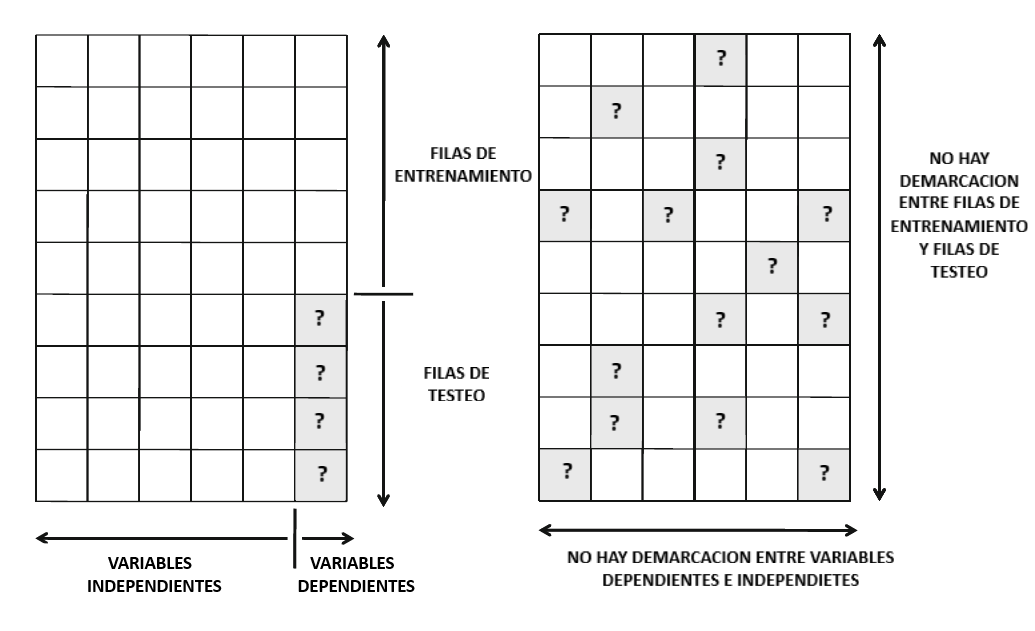
\includegraphics[width=0.8\textwidth]{CFvsRegresion.png}
\caption{A la izquierda una matriz usual en regresión y a la derecha la matriz del problema de filtrado colaborativo}\label{fig:CFvsReg}
\end{figure}

El problema del filtrado colaborativo se puede ver como una generalización de un problema de clasificación o regresión\cite{agg} \cite{cacheda2011comparison} \cite{vucetic2005collaborative} o como un caso especial del problema de valores faltantes (\textit{missing data}). En un problema de clasificación en general podemos pensar que la variable dependiente o clase a determinar, es en realidad un atributo con valores faltantes que queremos calcular, representados en una columna y todas las otras columnas son las variables independientes. En el caso del filtro colaborativo permitimos que los valores faltantes a predecir no son sólo un atributo, es decir solo una columna, sino que son varias diferentes y no pertenecen necesariamente a las mismas columnas, por lo cual no es posible identificar las variables dependientes de las independientes. En estos casos tiene mas sentido pensar en observaciones de entrenamiento y observaciones de testeo que en filas de entrenamiento y testeo como es en el caso de la clasificación/regresión. En la figura \ref{fig:CFvsReg} podemos ver la comparación entre la clasificación y los filtros colaborativos, donde las posiciones con signos de interrogación representan los valores desconocidos.

A la hora de elegir algún método de estos debemos tener claro cual es el objetivo del algoritmo así como su diseño, para que una mejora en la métrica refleje verdaderamente una mejora en la efectividad del mismo. En lineas generales, los dos principales tareas que se plantean los sistemas de recomendación son los siguientes:

\begin{itemize}
\item \textbf{Predicción} Este es el más simple de los objetivos y la formulación primitiva de un sistema de recomendación, predecir la valoración desconocida $r_{uj}$ del usuario $u$ sobre el ítem $j$ como $\hat{r}_{uj}$.

\item \textbf{Recomendación} En la mayoría de las configuraciones prácticas, el sistema no necesariamente busca las valoraciones o ratings específicos de los pares desconocidos usuario-ítem. En vez de esto, se busca	hallar los $k$ items más relevantes para un usuario en particular, o los $k$ usuarios más relevantes para un artículo en particular. Esta tarea es denominada como la recomendación \textit{top-k} de items o de usuarios. En general es mas común el escenario de recomendación de items que de usuarios. En algoritmos de recomendación tradicionales, el "problema top-k" casi siempre se refiere al proceso de búsqueda de los items \textit{top-k}, en lugar de los usuarios \textit{top-k} \cite{agg}.
\end{itemize}

\begin{figure}[htp]
\centering
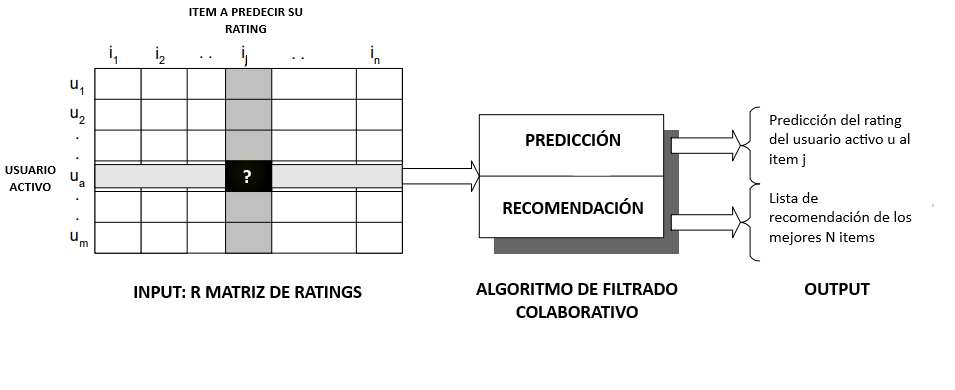
\includegraphics[width=0.9\textwidth]{procesoCF.png}
\caption{Esquema del proceso del filtrado colaborativo}
\label{fig:procesoCF}
\end{figure}

Los dos problemas antes mencionados están estrechamente relacionados\cite{agg}. Por ejemplo, para determinar los elementos top-k para un usuario en particular, uno puede predecir los ratings de cada ítem para ese usuario y tomar los $k$ elementos con las mejores valoraciones predichas. Sin embargo, los dos problemas no son necesariamente el mismo, de esto hablaremos mas adelante cuando discutamos las formas de medir el rendimiento de un sistema.

Existen otros objetivos secundarios que suelen complementar a las tareas recién descritas, algunas de ellas son la novedad de los items, la diversidad, la cobertura y la serendipia entre otros \cite{evaluateshani}. Aun así, estos últimos objetivos son difíciles de cuantificar y su evaluación suele ser muy subjetiva a cada sistema, por lo cual en el alcance de esta tesis nos limitaremos a utilizar las métricas mas generales que midan la precisión en la predicción de los ratings y rankings.


%%%%%%%%%%%%%%%%%%%%%%%%%%%%%%%%%%%%%%%%%%%%%%%%%%%
%%%%%%%%%%%%%%% SECCION CF %%%%%%%%%%%%%%%%%%%%%%%%
\section{Métricas de evaluación}

Dentro de la literatura de los sistemas de recomendación existen múltiples métricas utilizadas para evaluar su calidad como puede verse en la bibliografía \cite{agg} \cite{evaluateshani} \cite{evaluate-hertlocker}. La evaluación de un sistema se puede realizar en dos instancias diferentes, una \textit{online} y otra \textit{offline}. La primera de estas requiere necesariamente de interacción con los usuarios para obtener los resultados y aplicar técnicas del estilo de \textit{A/B testing} para comparar los mismos. Por otro lado, la evaluación offline utiliza datos históricos en general ya estandarizados, que contienen pares de usuario-items de los cuales se conocen los ratings. La evaluación offline es la más utilizada para comparar técnicas entre sí \cite{agg} debido a la estandarización de los conjuntos de datos públicos existentes para testeo como son \textit{Jester}, \textit{MovieLens} y \textit{Netflix} entre otros\cite{chen2012collaborative}. Para ampliar en técnicas de evaluación online se puede ver \cite{evaluateshani} \cite{kohavi2009controlled}.

La evaluación offline de la precisión de un sistema la podemos dividir en dos tipos de tareas diferentes según el objetivo de nuestro sistema, medir la precisión de los ratings que fueron predichos o la precisión del ranking de los items recomendados. Esta última se basa en el hecho de que podemos mirar solo el orden en el que se recomiendan los items sin tener en cuenta el rating de los mismos de forma explícita. A continuación describiremos brevemente las medidas consideradas con sus ventajas y desventajas.

\subsection{Medidas de predicción de ratings}

Las medidas de predicción de ratings son las más populares y más usadas debido a su simplicidad matemática y algorítmica. La idea de fondo detrás de las mismas es la suposición de que un usuario preferirá un algoritmo que pueda predecir sus ratings en general con mas precisión. Sea $S$ el conjunto de los ratings observados y sea $T \subset S$ un subconjunto de estas entradas conocidas que utilizaremos para el testeo del algoritmo. La elección de este conjunto puede ser aleatoria o utilizando una validación cruzada de $10$ o más iteraciones (\textit{K-fold cross-validation}) como describiremos más adelante.

Dado $r_{ui} \in T$ haremos un pequeño abuso de notación al utilizar $(u,i) \in T$ en su lugar, definimos el error $e_{ui}=r_{ui}-\hat{r}_{ui}$	donde $\hat{r}_{ui}$ representa el rating predicho. Entonces definimos el error cuadrático medio o MSE (\textit{Mean Squared Error}) por sus siglas en inglés y respectivamente la raíz del error cuadrático medio (RMSE)

\begin{definicion}
Definimos el MSE y el RMSE como:

\begin{align}
  MSE =& \frac{\sum_{(u,i)\in T} e_{ui}^2}{|T|} \\
  RMSE =& \sqrt{\frac{\sum_{(u,i)\in T} e_{ui}^2}{|T|}}
\end{align}
\end{definicion}

En esta tesis, utilizaremos el  término error cuadrático medio para referirnos al RMSE. Ademas otra métrica muy utilizada que definiremos es el error medio absoluto o MAE(\textit{Mean Absolute Value}).

\begin{definicion}
Definimos el MAE como:
\begin{equation}
MAE = \frac{\sum_{(u,i)\in T} \abs{e_{ui}}}{|T|}
\end{equation} 
\end{definicion}

Claramente valores mas pequeños del RMSE y MAE significan errores más pequeños en los ratings estimados y por lo tanto mejor predicción de los ratings. Consideraremos también la versión normalizada de estas métricas, NRMSE y NMAE las cuales resultan de dividir las mismas por la longitud del rango de ratings $(r_{min},r_{max})$ que nos permiten garantizar que nuestras métricas estén dentro del intervalo $(0,1)$.

¿Cuál de estas métricas es mejor? En general no hay una respuesta definitiva a esta pregunta y dependemos de la aplicación del algoritmo de recomendación. El RMSE tiende a penalizar fuertemente errores muy grandes debido a que los eleva al cuadrado en comparación al MAE, en la competencia \textit{The Netflix Prize} se utilizo el RMSE\cite{bennett2007netflix}. Se puede encontrar una discusión mas profunda acerca de las ventajas y desventajas entre ambas métricas en Willmott et al. \cite{RMSEwillmott2005advantages} y Chai et al. \cite{RMSEchai2014root}.

%la metrica mas estandar, el RMSE, utilizada en el concurso de Netflix Prize(CITA).

%(\colorbox{LimeGreen}{ACA PREGUNTAR SI CONVIENTE TAMBIEN AGREGAR MAE})

%En general las medidas de precision en la prediccion de ratings o tambien llamadas basadas en error, son utilizadas para la seleccion de los hiperparametros del modelo y luego se utilizan otras metricas mas costosas o mas especificas para elegir el algoritmo.

\subsection{Medidas de predicción de rankings}

Tanto el RMSE como el MAE, tienen en cuenta todos los errores realizados sobre los ratings predichos, pero en muchas aplicaciones de los sistemas de recomendación no tienen como objetivo la estimación de los ratings en sí, sino en una recomendación de una lista de $k$ elementos de mayor interés para el usuario. Bajo este contexto, dentro de la teoría de la recuperación de información (\textit{Information Retrieval}), existen múltiples métricas para evaluar este tipo de problemas que dependen del tipo de rating de los items, ya sea un sistema de evaluación binaria (por ejemplo compras, clicks, etc.) o de múltiples valores (puntuación, rating, etc.).

\subsubsection{Precision-Recall y MAP}

Llamaremos $usuario$ $activo$ al usuario $u$ al cual se le realizará la recomendación, llamemos $M_u(k)$ al \textit{top-k} de items recomendados por nuestro sistema para ese usuario. Sea $I_u$ el conjunto de items evaluados por el usuario activo, cada uno de esos items, podemos clasificarlos como relevantes para este usuario o no a partir de algún valor de corte. Por ejemplo en un caso de un rating del 1 al 5, podría depender de la media de los ratings del usuario o ser un valor fijo. A la vez, dados los items $j\in M_u(k)$, diremos que esos items son recomendados si el rating estimado $\hat{r}_{uj}$ también es mayor al corte determinado. Resumiendo, si elegimos un valor de corte para los ratings $\delta > 0$:

\begin{eqnarray*}
i\in I \text{ es relevante para } u \Longleftrightarrow& r_{ui} \geq \delta \\
i \in I \text{ es recomendado para } u \Longleftrightarrow& \hat{r}_{ui} \geq \delta \text{ e } i \in M_u(k)
\end{eqnarray*}

Por lo tanto, podemos definir para cada usuario $u$, a $G_u \subset I_u$ como el conjunto de todos los items relevantes para este usuario. Además definiremos una indicadora para el usuario activo y un ítem $i\in M_u(k)$, que marcará cuándo efectivamente recuperamos un ítem relevante en la recomendación:

\begin{equation*}
\text{Rel}_u(i) = 
\begin{cases}
1, &\text{si  } r_{ui} \geq \delta \wedge \hat{r}_{ui} \geq \delta \\
0, &\text{si no}
\end{cases}
\end{equation*}

\begin{definicion}
Definimos la precision ($P_{u}(k)$ o \textbf{P@k}) y la exhaustividad (\textit{Recall}, $R_{u}(k)$ o \textbf{R@k}) en $k$ como:

\begin{align}
P_{u}(k) &= \frac{|S_u(k) \cap G_u|}{|S_u(k)|} \\
R_{u}(k) &= \frac{|S_u(k) \cap G_u|}{|G_u|}
\end{align}
\hfill$\square$
\end{definicion}

La precisión $P(k)$\footnote{En general haremos un abuso de notación, utilizando $P(k)$ en lugar de $P_u(k)$ cuando se entiende que esta fijo el usuario. Respectivamente, haremos lo mismo con $R_u(k)$ y $S_u(k)$} para un usuario $u$, mide el porcentaje de items recomendados en el top-$k$ que son relevantes para el usuario activo y la exhaustividad, $R(k)$, mide el porcentaje del total de los items relevantes que han sido recomendados. 

Una manera fácil de interpretar estas medidas es pensar que los items relevantes y que son recomendados a la vez, son los resultados verdaderos positivos (True-Positive) conseguidos en $S_u(k)$ como en el cuadro \ref{t:recomvsrel}, entonces la precisión debería ser el resultado de dividir estos resultados verdaderos positivos sobre todos los recomendados en $S_u(k)$, es decir los Verdaderos-Positivos (TP) más los Falsos-Positivos(FP). Análogamente podemos definir el recall, resultando entonces:

\begin{align}
P(k) &= \frac{TP}{TP + FP} \\
R(k) &= \frac{TP}{TP + FN}
\end{align}

Generalmente buscamos un equilibrio entre estas cantidades ya que, por ejemplo, recomendar más items puede perder precisión, pues esta no es monótona, pero a la vez captura mas elementos relevantes que antes, mejorando el recall. Para poder analizar este intercambio podemos graficar lo que se conoce como la curva \textit{precision-recall}, mas adelante hablaremos de las mismas. 

\begin{table}[htb]
\begin{center}
\begin{tabular}{|c|c|c|}
\hline
  & Recomendado & No recomendado \\
\hline
Relevante & True-Positive (TP) & False-Negative (FN)\\
\hline
No Relevante & False-Positive (FP) & True-Negative (TN)\\
\hline
\end{tabular}
\caption{Representación de los posibles resultados de las recomendaciones/relevancia.}\label{t:recomvsrel}
\end{center}
\end{table}

La precisión es una medida muy utilizada debido a su clara interpretación, pero posee algunas desventajas, por ejemplo, si el usuario elegido no poseía items relevantes, el valor de $P(k)$ no será informativo. Además la precisión no valora el orden en el cual los items son recomendados, dentro del conjunto de items recomendado solo evalúa si son relevantes o no. Por este motivo introducimos la \textit{Media de la Precisión Promedio} o \textbf{MAP} por sus siglas en ingles (\textit{Mean Average Precision}) que calcula la precisión de la lista de longitud $l$ donde $l=1,\ldots, k$ y los promedia y luego nuevamente promedia pero sobre todos los usuarios. Con este motivo, primero introduciremos la precisión promedio:

\begin{definicion}
Fijado el usuario activo $u$, sea $m_{u}=|G_u|$ como la cantidad de items valorados que son relevantes, llamaremos \textit{precision promedio} en $k$ ($AP_u(k)$ o AP@k) como:
\begin{equation}
AP_u(k)= \frac{1}{\min(k,m_{u})} \sum_{l=1}^{k} P_{u}(l) \cdot \text{Rel}(l)
\end{equation}
Donde el término $\min(k,m_{u})$ normaliza sobre la cantidad de items relevantes, pero previniendo que sea fuertemente penalizada la métrica en caso de que la cantidad de items a recomendar fuera mucho menor a los items relevantes.
\end{definicion}

A diferencia de las métricas de precisión de rating vistas(RMSE y MAE), para las cuales un valor menor en la métrica significa una mejor predicción, la precisión promedio, al igual que la precisión y el recall, un mayor valor de las mismas significa una mejor predicción del ranking. En el caso de la precisión y el recall en $k$, el valor máximo que pueden alcanzar es 1, aunque no siempre lo alcanzaran.
%%% Lema: AP<=1

\begin{definicion}
Sea $n$ la cantidad total de usuarios, definimos el promedio de la precisión promedio(MAP) en $k$  como:

\begin{equation}
\label{err:map}
\textbf{MAP@k} = \frac{1}{n} \sum_{u=1}^{n} AP_u(k)
\end{equation}
\end{definicion}

Una de las ventajas de MAP es que no solo genera una medida global sobre todos los usuarios, sino que le otorga mayor importancia al orden en el cual los items fueron recomendados al estar basado en la precisión promedio.

\begin{ejemplo}
Supongamos que tenemos un sistema de recomendación de libros donde aplicaremos dos algoritmos diferentes, A y B, y un tercer algoritmo perfecto C para contrastar los anteriores. Queremos evaluar su rendimiento para recomendar ocho libros a un usuario activo y para eso compararemos su precision, recall y MAP. Supongamos que hay solo tres items relevantes entre los disponibles para el usuario $m_u$ y los resultados obtenidos son los siguientes: 

\begin{table}[htb]
\begin{center}
\begin{tabular}{|c|c c c|c c c|c c c|}
\hline
\multicolumn{1}{|c|}{} & \multicolumn{3}{| c |}{Algoritmo A} & \multicolumn{3}{| c |}{Algoritmo B} & \multicolumn{3}{| c |}{Algoritmo C}\\
\hline
\multicolumn{1}{|c|}{Ranking($i$)} & Rel & P(i) & R(i) & Rel & P(i) & R(i)& Rel & P(i) & R(i)\\
\hline
1 & 1 & 1/1 & 1/3 & 1 & 1/1 & 1/3 & 1 & 1/1 & 1/3 \\
2 & 1 & 2/2 & 2/3 & 0 & 1/2 & 1/3 & 1 & 2/2 & 2/3 \\
3 & 0 & 2/3 & 2/3 & 0 & 1/3 & 1/3 & 1 & 3/3 & 3/3 \\
4 & 1 & 3/4 & 3/3 & 1 & 2/4 & 2/3 & 0 & 3/4 & 3/3 \\
5 & 0 & 3/5 & 3/3 & 0 & 2/5 & 2/3 & 0 & 3/5 & 3/3 \\
6 & 0 & 3/6 & 3/3 & 0 & 2/6 & 2/3 & 0 & 3/6 & 3/3 \\
7 & 0 & 3/7 & 3/3 & 0 & 2/7 & 2/3 & 0 & 3/7 & 3/3 \\
8 & 0 & 3/8 & 3/3 & 1 & 3/8 & 3/3 & 0 & 3/8 & 3/3 \\
\hline
\end{tabular}
\end{center}
\end{table}

Notemos que si solo tomasemos en cuenta $P(8)$ y $R(8)$, la última fila del recuadro, tendíamos que el rendimiento de los tres algoritmos es el mismo, pero es claro que el algoritmo C, el perfecto, tiene mejor rendimiento en conseguir recomendar de manera óptima los libros, ya que son los tres primeros que recomendo. Por ejemplo si tomásemos $P(3)$ y $R(3)$, se ve claramente como el algoritmo C es superior al A y al B. Calculemos ahora la precisión promedio para cada algoritmo, donde si $Rel(i)=0$ no aportará a la métrica:

\begin{eqnarray*}
AP^{(A)}(8)=& (1 \cdot 1 + \frac{2}{2} \cdot 1 + \frac{3}{4} \cdot 1) \times \frac{1}{3} \approx 0.92 \\
AP^{(B)}(8)=& (1 \cdot 1 + \frac{2}{4} \cdot 1 + \frac{3}{8} \cdot 1) \times \frac{1}{3} \approx 0.62 \\
AP^{(A)}(8)=& (1 \cdot 1 + \frac{2}{2} \cdot 1 + \frac{3}{3} \cdot 1) \times \frac{1}{3} = 1
\end{eqnarray*}

Ahora queda claro que el mejor rendimiento entre los dos algoritmos A y B, es el del A, lo cual era evidente ya que conseguía en las primeras 4 recomendaciones pegarle a los tres libros relevantes, mientas que el B solo conseguía recomendar dos de ellos y recién en la octava recomendación conseguía el libro relevante restante.  

\end{ejemplo}

%%%%%%%%%%%%%%%%%%%%%%%%%%%%%%%%%%%%%%%%%%%%
\subsubsection{Métricas basadas en utilidad}

Las métricas basadas en utilidad hacen uso tanto de los ratings conocidos de los usuarios, como del ranking de recomendación del sistema. En general estas métricas utilizaran alguna función de ganancia que involucra ambas cosas, rating y ranking. Definiremos tres métricas muy utilizadas en este aspecto, $R$-$Score$, $NDCG$ y el $ARHR$.

Consideremos el conjunto $I_u$ de los items valuados por el usuario $u$, para el ítem $j$ definimos la utilidad basada en rating como el $\max\{r_{uj}-C_u,0\}$ donde $C_u$ es un punto de corte para el usuario $u$ que puede ser definido como la media de los items que evaluó y sea $v_j$ el ranking del ítem $j$ en la lista de recomendación de nuestro sistema para nuestro usuario activo. Dado $\alpha$ un parámetro de ajuste, definimos entonces la utilidad del par $(u,j)$ como:

\begin{equation}
F(u,j) = \frac{\max\{r_{uj}-C_u,0\}}{2^{{(v_j-1)}/\alpha}}
\end{equation}

Y definimos entonces para cada usuario lo que se conoce como \textit{R-score}(u) y el \textit{R-score} global como:

\begin{align}
\text{R-score(u)} &= \sum_{j \in I_u} F(u,j)\\
\text{R-score} &= \sum_{u} \text{R-score}(u)
\end{align}

El término $2^{-{(v_j-1)}}$ generalmente conocido como la utilidad basada en el ranking, asegura una caída exponencial en el mismo bajo la lógica de que un usuario estará mas interesado en los items rankeados mas alto que en los últimos recomendados. Sin embargo, esto depende mucho del contexto del sistema de recomendación y la cantidad de elementos recomendados en la lista.

A continuación, introduciremos una métrica que penaliza menos el ranking que el R-score. Sea $g_{uj}$ una función de utilidad del usuario $u$ sobre el ítem $j$, típicamente se define como una función exponencial del ranking o relevancia como por ejemplo:

\begin{equation}
g_{uj} = 2^{rel_{uj}}-1
\end{equation}

Aquí la relevancia ($rel_{uj}$) del ítem $j$ para el usuario $u$ esta representada por el valor verdadero de su rating\cite{NDCGweimer2008cofi}. También se suele utilizar como función de ganancia lineal a la misma relevancia $g_{uj}=rel_{uj}$, que a diferencia de la función exponencial, no le da un peso tan grande a los items de mayor relevancia. Consideremos ahora un término de descuento o penalización sobre el orden en el que aparecen los items, en general se utiliza un función creciente logarítmica que penalice esa ganancia como $\log_2 (j+1)$. De esta forma, penalizamos items relevantes que aparezcan bajos en el orden de recomendación. 

\begin{definicion}
Definimos la Ganancia Acumulada Descontada o Discounted Cumulative Gain (\textit{DCG}) sobre todos los usuarios y su versión normalizada (\textit{NDCG}) como:
\begin{eqnarray}
DCG =& \frac{1}{n} \sum_{u=1}^{n} \sum_{j \in I_u} \frac{g_{uj}}{\log_2(j+1)}\\
NDCG =& \frac{DCG}{IDCG}
\end{eqnarray}
\end{definicion}

Donde el IDCG es el Ideal Discounted Cumulative Gain, que se calcula con el DCG pero en vez de utilizar la relevancia de los rankings predichos, utilizamos el orden de la recomendación óptima para el usuario. El NDCG se encuentra entre $[0,1]$, siendo 1 el valor óptimo de esta medida, y al igual que con la precisión, mientas mayor sea esta métrica, mejor será el rendimiento. En general utilizaremos la versión normalizada pero calculada sólo sobre los items en la recomendación top-k y promediaremos sobre todos los usuarios:

\begin{equation}
DCG(k) = \frac{1}{n} \sum_{u=1}^{n} \sum_{j \in I_u,j\leq k} \frac{2^{rel_{uj}}-1}{\log_2(j+1)}
\end{equation}

\begin{equation}
\label{err:ndcg}
NDCG(k) = \frac{DCG(k)}{IDCG(k)}
\end{equation}

Por último  definimos el Average Reciprocal Hit-Rate (\textit{ARHR}) o también conocido como Mean Reciprocal Rank (\textit{MRR}) como:

\begin{equation}
ARHR(u) = \sum_{j \in I_u} \frac{rel_{uj}}{v_j} 
\end{equation}

En este caso el $rel_{uj}\in \{0,1\}$ representa si el ítem es relevante o no, nuevamente dependiendo de algún punto de corte. Entonces el ARHR global es:

\begin{equation}
ARHR = \frac{1}{n}{\sum_{u=1}^{n} ARHR(u)}
\end{equation}

\begin{ejemplo}
Supongamos que tenemos un sistema de recomendación de películas en el cual las mismas son evaluadas del 0 al 3. Supongamos que queremos evaluar el rendimiento en el top-6 del sistema con la métrica NDCG de ganancia exponencial. Supongamos que el sistema recomienda en orden descendente de preferencia las películas $F_1,\cdots,F_6$. Primero calculemos el DCG, para esto necesitamos los verdaderos ratings $r_{ui}$ que el usuario había dado a los items que el sistema recomendo, y sobre eso calculamos la ganacia y el descuento:

\begin{center}
\begin{tabular}{|c|c|c|c|c|c|}
\hline
Ranking & Película & Rating & Ganancia & Descuento \\
\hline
1 & $F_1$ & 3 & 7 & 1  \\
\hline
2 & $F_2$ & 2 & 3 & 1.585  \\
\hline
3 & $F_3$ & 3 & 7 & 2 \\
\hline
4 & $F_4$ & 0 & 0 & 2.322  \\
\hline
5 & $F_5$ & 1 & 1 & 2.585  \\
\hline
6 & $F_6$ & 2 & 3 & 2.807  \\
\hline
\end{tabular}
\end{center}

Por lo tanto el DCG(6) = $7+(\frac{3}{1.585})+(\frac{7}{2})+(\frac{0}{2.322})+(\frac{1}{2.585})+(\frac{3}{2.807})\approx 13.848$\\
El valor del DCG solamente no parece ser muy informativo sin una referencia, para lo cual calculamos el IDCG para poder normalizar el valor de la métrica. Asumamos que el orden real de las 6 películas preferidas del usuario eran $\{F_1,F_3,F_7,F_2,F_6,F_9\}$, donde aparecen películas que el sistema no había recomendado como la $F_7$ y la $F_9$ con $r_{u,7}=3$ y $r_{u,9}=1$ respectivamente:

\begin{center}
\begin{tabular}{|c|c|c|c|c|c|}
\hline
Ranking & Película & Rating & Ganancia & Descuento \\
\hline
1 & $F_1$ & 3 & 7 & 1  \\
\hline
2 & $F_3$ & 3 & 7 & 1.585  \\
\hline
3 & $F_7$ & 3 & 7 & 2 \\
\hline
4 & $F_2$ & 2 & 3 & 2.322  \\
\hline
5 & $F_6$ & 2 & 3 & 2.585  \\
\hline
6 & $F_9$ & 1 & 1 & 2.807  \\
\hline
\end{tabular}
\end{center}

Entonces IDCG(6) = $\frac{7}{1}+\frac{7}{1.585}+\frac{7}{2}+\frac{3}{2.322}+\frac{3}{2.585}+\frac{1}{2.807}\approx 17.725$, y por lo tanto:

\begin{equation}
NDCG(6)=\frac{DCG(6)}{IDCG(6)}=\frac{13.848}{17.725} \approx 0.718
\end{equation}

Dandonos así una métrica estandarizada, que nos permite tener una mejor idea que tan cerca estuvo nuestro sistema de recomendar de manera óptima las películas. \hfill$\square$
\end{ejemplo}



%%%%%%%%%%%%%%%%%%%%%%%%
%% Poner curvas ROC y AUCROC?
%% Curva precision-recall?
%%%%%%%%%%%%%%%%%%%%%%%%

%%%%%%%%%%%%%%%%%%%%%%%%%%%%%%%%%%%%%%%%%%%%%%%%%%%%%%%%%%%%%%%%%%%%%%%%%%%%
%%%%%%%%%%%%%%%%%% Técnicas %%%%%%%%%%%%%%%%%%%%%%%%
\section{Técnicas clásicas de filtros colaborativos}

En esta sección desarrollaremos algunas las técnicas más populares dentro de los filtros colaborativos como SVD y \textit{Slope One}, y otras más actuales como son las Máquinas de Factorización. Describiremos como se establecen las predicciones de los ratings y cuales son sus ventajas y desventajas.

Recordemos algunos aspectos de la notación y definiciones que utilizaremos en general:

\begin{itemize}
\item Sea ${U}=\{u_1,u_2,\cdots,u_n\}$  la lista de los $n$ usuarios.
\item Sea ${I}=\{i_1,i_2,\cdots,i_m\}$  el conjunto de los $m$ items.
\item Sea $R$ la matriz de ratings usuarios-items con los ratings observados apartados para el entrenamiento del algoritmo, en las posiciones dadas por $\mathcal{K}$ y el resto de las posiciones como desconocidas. Separaremos en un principio los datos observados $S$ en dos conjuntos disjuntos $E$ y $T$, donde $E$ es el conjunto de datos de entrenamiento para el algoritmo y $T$ es el conjunto de datos para el testeo. En general la proporción de datos reservados para testeo será entre un 20\% y un 25\% del total de los datos.
\end{itemize}

%%%%%%%%%%%%%%%%%%%%%%%%%%%%%%%%%%%%%%%%%%%%%%%%%%%%%%%%%%%%%%%%%%%%%%%%%%%

\subsection{\texorpdfstring{$k-$}-Vecinos mas cercanos}

Los algoritmos basados en vecindades tienen su fundamento en la hipótesis de que si dos usuarios tienen un comportamiento similar a la hora de evaluar los mismos items, entonces probablemente podamos usar esa información para predecir el comportamiento de un usuario sobre un ítem no evaluado a partir de los usuarios parecidos. Este razonamiento se puede hacer de forma análoga para los items que son similares entre si, entonces podemos definir dos acercamientos diferentes \cite{neighbordsurvey}:

\begin{itemize}
\item \textit{Modelos basados en usuarios}: usuarios similares tendrán similares gustos por el mismo ítem. Por ejemplo, si dos usuarios A y B evaluaron los mismos items de manera muy similar excepto por un solo ítem $i$ que solo evaluó A, entonces tendría sentido utilizar ese rating para estimar el rating de B sobre $i$.
\item \textit{Modelos basados en items}: items similares serán evaluados de forma similar por el mismo usuario.
\end{itemize}

Una vez definido que modelo utilizar, nosotros utilizaremos un modelo basado en items, supondremos que queremos estimar el rating del usuario activo $u$ sobre el ítem activo $j$, el algoritmo lo podemos desglosar en tres pasos\cite{herlocker1999algorithmic}:

\begin{enumerate}
\item Calcular la similitud entre el ítem $j$ activo y el resto de los items.
\item Seleccionar un subconjunto de esos items como $vecindad$ del ítem activo.
\item Utilizando los ratings de la vecindad del ítem activo, predecir el rating del usuario activo para el ítem $j$.
\end{enumerate}

Para definir la vecindad necesitaremos fijar un parámetro $k\in \mathbb{N}$, entonces la vecindad será $N_j(u)=\{i_1,i_2,\dots,i_k\}$ el conjunto de los k items que mas se parecen a $j$, que han sido evaluados por el usuario $u$. Esta forma de definir la vecindad es la que caracteriza a esta técnica, conocida por sus siglas en inglés como k-NN por \textit{k-Nearest Neighbours}.

% Sea la matriz de ratings $R=[r_{uj}]$ con $u=\{1,2,\dots,N\}$ y $j=\{1,2,\dots,M\}$ y supongamos en un principio que las entradas faltantes son cero\footnotemark con el propósito de facilitarnos el modelo. Sea $\mathcal{K}$ el conjunto de entradas conocidas de la matriz R, es decir las especificadas por los usuarios. 

\subsubsection{Cálculo de similitud}
Existen múltiples formas de evaluar la similitud entre dos items o entre dos usuarios\cite{cacheda2011comparison}\cite{neighbordsurvey}, nosotros describiremos dos en particular, el \textit{índice de correlación de Pearson} y la \textit{similitud coseno}, ambas medidas de las mas utilizadas\cite{agg}\cite{herlocker1999algorithmic}\cite{sarwar2001item}. Sea $u$ el usuario activo y supongamos que queremos predecir el rating $\hat{r}_{uj}$ para un ítem $j$, para esto tenemos que establecer la similitud entre el ítem activo y otro ítem $i$. Consideremos $U_i$, $U_j$ los conjuntos de los usuarios que evaluaron cada ítem respectivamente en el conjunto de entrenamiento $E$, las dos medidas de similitud consideradas se pueden definir de la siguiente manera:

\begin{definicion}
Dados dos items $i$ y $j$, definimos la similitud coseno como:

\begin{equation}
\text{Sim}^{(C)}(i,j)= Cos(i,j) = \frac{\sum_{v \in {U_i\cap U_j}} r_{vi} \cdot r_{vj}}{{\sqrt{\sum_{v \in {U_i\cap U_j}} r_{vi}^2}}{\sqrt{\sum_{v \in {U_i\cap U_j}} r_{vj}^2}}}
\end{equation}
\end{definicion}

Antes de definir la correlación de Pearson, definimos $\mu_i$ como el promedio de los ratings sobre $i$:

\begin{equation}
\mu_j =\frac{1}{|U_j|} \sum_{v \in U_j} r_{vj}
\end{equation}

\begin{definicion}
Consideremos $\mu_i$ el promedio de los ratings que recibió el ítem $i$, definimos la similitud entre dos items como el indicie de \textit{correlación de Pearson}:

\begin{equation}
\text{Sim}^{(P)}(i,j) = Pearson(i,j) = \frac{ \sum_{v \in {U_i\cap U_j}} (r_{vi}-\mu_i)(r_{vj}-\mu_j) }{{\sqrt{\sum_{v \in {U_i\cap U_j}} (r_{vi}-\mu_i)^2}}{\sqrt{\sum_{v \in {U_i\cap U_j}}(r_{vj}-\mu_j)^2}}}
\end{equation}
\end{definicion}

Es clara la interpretación de estas similitudes, si pensamos a los items representados como un vector $\vec{R}_{-,i} \in \mathbb{R}^n$ que es la columna i-ésima de la matriz $R$ donde los datos faltantes los tratamos como 0, entonces por ejemplo la similitud coseno coincide con el coseno del ángulo $\theta_{ij}$ comprendido entre los vectores que representan ambos items, podemos entonces reescribirla como:

\begin{equation}
Cos(i,j) = \cos (\theta_{ij}) =\frac{\vec{R}_{-,i} \cdot \vec{R}_{-,j}}{\norm{\vec{R}_{-,i}} \norm{\vec{R}_{-,ij}}}
\end{equation}

Con $\norm{.} = \norm{.}_2$
%Sea $\sigma_i$ es el desvío estándar calculado sobre los usuarios que evaluaron dicho ítem:
%\begin{equation}
%\sigma_i=\sqrt{\frac{\sum_{v \in {U_i}}{(r_{vi}-\mu_i)^2}}{|{U_i}|-1}}
%\end{equation}

\subsubsection{Calculo de predicción}
Finalmente resta calcular ahora la predicción del rating $\hat{r}_{uj}$ sobre el ítem $j$, para eso recordemos que $N_j(u)$ es el conjunto de k items más parecidos a $j$ que han sido evaluados por $u$. Entonces la predicción P(u,j) que consideraremos será una suma pesada:

\begin{equation}
P(u,j) = \hat{r}_{uj}=\frac{\sum_{i \in N_j(u)}\text{Sim(i,j)} \cdot r_{ui}}{\sum_{i \in N_j(u)}|\text{Sim(i,j)}|}
\end{equation}

La motivación detrás de esta suma es pesar sobre los propios ratings que ya proporciono el usuario para los items similares, ya que dichos ratings son predictores más confiables.

En el cuadro \ref{alg:knn} podemos ver el pseudocódigo en forma general de este algoritmo basado en items.

\begin{algorithm}[H]
\begin{algorithmic}[KNN]
\REQUIRE $E=$ conjunto de entradas de entrenamiento, $k$, $u$ usuario activo, $j$ ítem activo 
\ENSURE Predicción $\hat{r}_{uj}$
\FORALL {$i \in I$}
\STATE $\mu_i \leftarrow \frac{1}{|U_j|} \sum_{v \in U_j} r_{vj}$
\STATE Calcular Sim(i,j)
\ENDFOR
\STATE Calcular $N_j(u)$
\STATE $\hat{r}_{uj} \leftarrow P(u,j)$
\end{algorithmic}
\caption{k-NN}\label{alg:knn}
\end{algorithm}

\subsubsection{Variantes}

Existen muchas variantes de este tipo de métodos, en general, las variantes más clásicas incluyen modificaciones en la forma del cálculo de la similitud, la forma del elegir el vecindario o como calcular la predicción\cite{sarwar2001item}. En el cálculo de la predicción es usual la utilización de pesos vinculados a la frecuencia relativa de los items. Dos variantes usuales en el cálculo de la predicción del rating son centrar en la media de los ratings y también el de realizar una normalización de los ratings(Z-score)\cite{agg}.

\subsubsection{Ventajas y desventajas del método}

Caben destacar algunos puntos que tienen a favor los métodos basados en vecindarios:

\begin{itemize}
\item Simplicidad: La implementación de estos métodos es relativamente sencilla y funciona de manera muy intuitiva, sin tener la necesidad de ajustar una gran cantidad de parámetros mas que el tamaño de los vecindarios.
\item Explicabilidad: El modelo en el que nos basamos es sencillo de interpretar, pero también de justificar. Por ejemplo, al usuario se le puede explicar que la recomendación de un ítem proviene de haber visto tales otros items.
\item Eficiencia y estabilidad: Los métodos basados en vecindarios son algorítmicamente poco costosos y rápidos de ejecutar. No solo eso sino que también son estables al agregar nuevos usuarios y nuevos items\cite{neighbordsurvey}.
\end{itemize}

Sin embargo, por otro lado, el alcance de esta técnica es limitado, ya que para poder calcular la similitud entre dos items(usuarios), dependemos de que estos hayan sido evaluados por varios usuarios al mismo tiempo, mientas que sabemos que dos items pueden ser similares aunque esto no haya sucedido. Además, dado que solo se pueden recomendar items clasificados por vecinos, la cobertura de tales métodos también puede ser limitada.

Además, hay que sumar a esto la sensibilidad a la gran cantidad de datos faltantes que en esta técnica nos son tenidos en cuenta, esto representa la mayor dificultad para los sistemas de recomendación en general. En este escenario es mas probable que dos usuarios(items) no tengan items evaluados en común, con lo cual nunca los podremos comparar, y así encontraremos pocos usuarios(items) parecidos.

%%%%%%%%%%%%%%%%%%%%%%%%%%%%%%%%%%%%%%%%%%%%%%%%%%%%%%%%%%%%%%%%%%%%%%
\subsection{Slope One}

El esquema llamado \textit{Slope One} desarrollado en \cite{slope} consiste en una técnica basada en un modelo de regresión. Supongamos que dados dos usuarios $u$ y $v$ con sus respectivos ratings dados como vectores filas de la matriz de ratings $R$, llamemoslos $R_u$ y $R_v$ respectivamente, donde cada elemento de cada uno de esos vectores es un rating de un ítem $i=1,2,\cdots,m$. La motivación de esta técnica es modelar la variación("diferencial") de la popularidad entre los items para los usuarios y luego utilizar esto como un predictor lineal para los ratings de un usuario. Veamos un ejemplo para entender la idea,

\begin{ejemplo}
Supongamos que tenemos tres items y dos usuarios A y B con los siguientes datos:

\begin{center}
\begin{tabular}{|c|c|c|c|}
\hline
 & ítem 1 & ítem 2 & ítem 3  \\
\hline
Usuario A & 3 & 5 & ? \\
Usuario B & 4 & 3 & 3 \\
\hline
\end{tabular}
\end{center}

Queremos predecir en este caso el rating del usuario A sobre el ítem 3, entonces lo que propone el método es mirar las diferencias de ratings para el otro usuario que conocemos B para modelar la variación de dichos items dentro de un mismo usuario. Las diferencias son:

\begin{eqnarray*}
Dif(B_3,B_1) &= 3 - 4 = -1\\
Dif(B_3,B_2) &= 3 - 3 = 0
\end{eqnarray*}

Luego propondremos para predecir el rating de A usar sus ratings sobre los otros items, modificados por esta diferencial de popularidad y promediaremos sobre todos los items que evaluó A, resultando:

\begin{equation*}
P(A_3) = \frac{(A_1 + Dif(B_3,B_1)) + (A_2 + Dif(B_3,B_2))}{2} = \frac{(3 +(-1)) + (5 + 0)}{2} = 3.5
\end{equation*}
\hfill$\square$
\end{ejemplo}

Formalmente, queremos hallar un  predictor lineal de la forma $f(x)=x+b$ para predecir los ratings de $v$ a partir de los ratings de $u$, de tal forma que minimice $\sum_{i} (r_{ui}-r_{vi})^2$. Derivamos e igualamos a cero y obtenemos $b=\sum_{i} \frac{r_{ui}+b-r_{vi}}{m}$ donde $m$ es la cantidad de items. 

Esto motiva la siguiente definición, consideremos $U_{ij}$ el conjunto de los usuarios que calificaron ambos items, sea el desvío promedio del ítem $i$ con respecto al ítem $j$ definido como:

\begin{equation}
\text{dev}_{ji}=\frac{1}{|U_{ij}|}\sum_{u \in U_{ij}} r_{uj}-r_{ui} 
\end{equation}

Entonces sea un ítem $i$ evaluado por $u$, resulta que $\text{dev}_{ji}+r_{ui}$ es un predictor para $r_{uj}$, por lo tanto es razonable definir al predictor de $r_{uj}$ como:

\begin{equation}
\hat{r}_{uj} = \frac{1}{|R_j^u|} \sum_{i \in R_j^u} \text{dev}_{ji}+r_{ui}
\end{equation}

Donde $R_j^u=\{i\in I_u | i\neq j,U_{ij}\neq \emptyset \}$ es el conjunto de items relevantes para $j$, es decir los items que fueron evaluados al menos una vez por un usuario que también evaluó a $j$. Finalmente queremos aproximar $\mu_u=\frac{1}{|I_u|}\sum_{i \in I_u} r_{ui} \approx \frac{1}{|R_j^u|}\sum_{i \in R_j^u} r_{ui}$, para esto necesitamos suponer que hay una cierta densidad en las evaluaciones de los datos, esto es que casi cualquier par de de items (i,j) fue evaluada al menos una vez. Si pedimos esto entonces $R_j^u=I_u$ si $j\notin I_u$ y $R_j^u=I_u-\{j\}$ si $j\in I_u$ y el predictor slope one $\hat{r}_{uj}^{S1}$, despejando $r_{ui}$, queda definido como:

\begin{equation}
\hat{r}_{uj}^{S1} =\mu_u + \frac{1}{|R_j^u|} \sum_{i \in R_j^u} \text{dev}_{ji}
\end{equation}

%%%%%%%%%%%%%%%%%%%%%%%%%%%%%%%%%%%%%%
\subsection{Factorización de matrices}

Los modelos de factores latentes como la factorización de matrices es un acercamiento totalmente diferente a los descritos previamente. Estas técnicas son consideradas parte del estado del arte en lo que a filtros colaborativos basados en modelos respecta\cite{agg} y tratan de capturar características(factores) latentes que expliquen las valoraciones de los items. La intuición para la aplicación de factorización de matrices es que las porciones de las filas y columnas de la matriz de ratings $R$ están altamente correlacionadas y como resultado, los datos tiene redundancias incorporadas, entonces la matriz de datos resultante a menudo se puede aproximar bastante bien por una matriz de bajo rango\footnotemark. 

\footnotetext{Para profundizar sobre la intuición detrás de la factorización de matrices se puede ver en Aggarwal et al\cite{agg}.}

La descomposición en valores singulares (SVD) ha demostrado ser un técnica útil en identificar factores latentes en semántica en el procesamiento natural del lenguaje\cite{koren2010factor}. Sin embargo, la principal dificultad en su aplicación en los sistemas de recomendación es la alta proporción de datos faltantes de la matriz $R$ de ratings de usuarios-items para la cual no esta definida la descomposición SVD tradicional. Frente a esta dificultad las primeras técnicas completaban la matriz para conseguir una matriz mas densa de ratings. El problema con este acercamiento es la complejidad algorítmica ya que incrementar la cantidad de información de la matriz lleva a un aumento muy significativo de los tiempos de ejecución del sistema de recomendación. Para evitar este inconveniente, en los trabajos mas recientes se realiza el modelado solo con los ratings observados $\mathcal{K}$, no solo mejorando los tiempos algorítmicos sino que también sorteando el problema de los datos faltantes. A continuación describiremos una de las técnicas más populares, la descomposición SVD regularizada.


\subsubsection{SVD}

Sea $R\in \mathbb{R}^{n\times m}$ la matriz de ratings usuarios-items, sabemos que podemos factorizar la matriz $R$ de forma aproximada como\footnotemark:
\footnotetext{El término SVD no es estrictamente correcto sino que se trata de una representación de bajo rango de la matriz $R$\cite{lu2015notes}. Sin embargo, en el área la utilización de este término para este tipo de factorización es ampliamente aceptada.}

\begin{equation}
R \approx PQ^T
\label{eq:SVD1}
\end{equation}

Donde $P\in \mathbb{R}^{n\times k}$ y $Q\in \mathbb{R}^{m\times k}$, y $k$ es un parámetro que representa la cantidad de factores latentes. La idea de trasfondo del método es que la i-ésima fila de P, que llamaremos el vector de factores del usuario, contiene las k entradas correspondientes a la afinidad del usuario $i$ hacia los $k$ factores latentes que intuitivamente representan algún concepto de los items. Las filas de Q son las representaciones a su vez de los $k$ conceptos de cada ítem. En este sentido $k$ es la dimensión del espacio de factores que codifican a las relaciones entre usuarios e items.

\begin{figure}[ht]
\centering
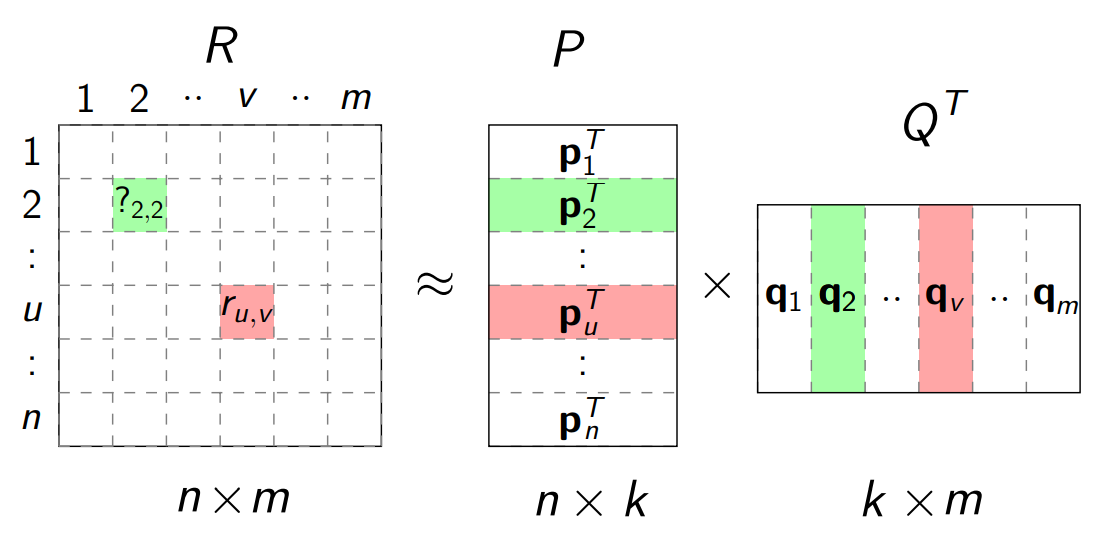
\includegraphics[width=0.8\textwidth]{MFpsota.png}
\caption{Representación de un modelo de factores latentes.}\label{fig:esquema-svd}
\end{figure}

Entonces si $R$ fuera una matriz densa se podría proponer el siguiente problema de optimización irrestricto:

\begin{equation}
\min_{\text{P, Q}}  \quad \frac{1}{2}\normbig{R-PQ^T}^2
\end{equation}

Donde $\norm{.}$ es la norma de Frobenius. Si llamamos $p_u\in\mathbb{R}^k$ a las filas de $P$ y $q_j\in\mathbb{R}^k$ a las filas de $Q$, podemos escribir el problema de manera equivalente como:

\begin{equation}
\min_{P_u,Q_j} \quad \frac{1}{2}\sum_{(u,j)}(r_{uj}- p_{u} \cdot q_{j}^T)^2=
\frac{1}{2}\sum_{(u,j)}(r_{uj}-\sum_{s=1}^k p_{ui} \cdot q_{ji})^2
\end{equation}

Planteado de esta forma, se pueden calcular $P$ y $Q$ mediante algún algoritmo de optimización irrestricto como el descenso por gradiente. Entonces la predicción del rating $\hat{r}_{uj}$  será:

\begin{equation}
\hat{r}_{uj} = \sum_{i=1}^k p_{ui} \cdot q_{ji}
\end{equation}

Este primer acercamiento supone, como primer dificultad, que se conocen todas las entradas de la matriz $R$, y aunque completemos la matriz de alguna forma, el otro problema que enfrentamos es la esparsidad, que puede llevar a que el modelo sobreajuste.

El método que consideraremos en esta tesis es el descrito en la sección 5.3.1 de \cite{korenadv} y mejorado en \cite{paterek2007improving}. En este modelo, la función a minimizar, estará calculada solo sobre las entradas calculadas de la matriz.

El modelo siempre trata de capturar de alguna manera las interacciones entre los usuarios y los items, pero suele haber efectos intrínsecos a cada usuario y a cada ítem que modifican su puntuación, podría ser que un usuario tenga tendencias a evaluar siempre altos los items mas que otros usuarios o que un ítem por su popularidad tenga mayor puntaje. Por esta razón es la que se introduce una predicción de base incluyendo sesgos para los usuarios $\{b_u:u\in {U}\}$ y para los items $\{b_j:j\in {I}\}$ y el promedio $\mu$ sobre todos los ratings observados:

Finalmente, introducideremos un término de regularización $\lambda>0$, para evitar el sobreajuste de los ratings. Entonces queda planteado el problema de aprender los parámetros como un problema de minimización que tiene como función de pérdida:

\begin{equation}
\label{eq:svd_biased}
\min_{b,p,q} \quad \sum_{(u,j)\in \mathcal{K}} (r_{uj}-\mu-b_u-b_j-p_u q^T_j)^2+\lambda (b_u^2+b_j^2+\norm{p_u}^2+\norm{q_j}^2)
\end{equation}

La optimización de la función de pérdida \eqref{eq:svd_biased} se realiza típicamente por medio del método de descenso por gradiente estocástico (\textit{stochastic gradient descent} SGD). Para lo necesitaremos elegir una tasa de aprendizaje $\alpha>0$, es decir el tamaño del paso del SGD, y alguna condición de convergencia bajo la cual terminar el algoritmo. Esta condición usualmente, depende de la cantidad de iteraciones o depender de la norma del error. En el recuadro Algoritmo \ref{alg:svdsgd} encontraremos el pseudocodigo del algoritmo SVD con SGD.

\begin{algorithm}[H]
\begin{algorithmic}[SGD]
\REQUIRE Matriz de ratings $R$, learning rate $\alpha$, $\lambda$ 
\ENSURE $b,p,q$
\STATE Iniciar aleatoriamente $b,p,q$
\STATE $\mathcal{K}=\{(u,j): \text{ entradas observadas}\}$
\WHILE {No se cumpla la condición de convergencia}
\STATE Reordenar aleatoriamente $\mathcal{K}$ en $S$
\FORALL {$(u,j) \in S$}
\STATE $e_{uj}=r_{uj}-\hat{r}_{uj}=r_{uj}-\mu-b_u-b_j-p_u^T q_j$
\STATE $b_u \leftarrow b_u + \alpha (e_{uj} - \lambda \cdot b_u)$
\STATE $b_j \leftarrow b_j + \alpha (e_{uj} - \lambda \cdot b_j)$
\STATE $p_u \leftarrow p_u + \alpha (e_{uj} \cdot q_j - \lambda \cdot p_u)$
\STATE $q_j \leftarrow q_j + \alpha (e_{uj} \cdot p_u - \lambda \cdot q_j)$
\ENDFOR
\STATE Calcular condición de convergencia
\ENDWHILE
\end{algorithmic}
\caption{SVD + SGD}\label{alg:svdsgd}
\end{algorithm}

La constante $\lambda$, que controla el nivel de la regularización y la tasa de aprendizaje, generalmente se determinan por validación cruzada. Los valores estipulados en \cite{korenadv} basados en la competencia de Netflix son $\lambda=0.02$ y $\alpha=0.005$.

\subsubsection{Variantes}
Una modificación sencilla para este algoritmo usualmente utilizada, es diferenciar el tamaño de los pasos que realiza el gradiente estocástico, introduciendo una tasa de aprendizaje independiente para cada variable así como un parámetro de regularización para cada variable. Introducir esta variación produce mejores resultados para la predicción\cite{takacs2007major}, al coste de un mayor tiempo de cómputo.

%% Si cuento SVD++ aunque sea de manera breve esto vuela
Se han aplicado numerosas mejoras a este algoritmo \cite{paterek2007improving}, pero entre ellas la variante más destacable, mostrando un rendimiento general superior a SVD, es el modelo desarrollado por Koren et al\cite{koren2008factorization} conocido como SVD++. Dicho sistema realiza una normalización sobre los ratings y luego utiliza un modelo basado en vecinos para mejorar el rendimiento del sistema. También se lo suele enmarcar dentro de una clase de modelos conocidos como \textit{factorización no negativa de matrices}\cite{agg}.

\subsubsection{Ventajas y desventajas}

La principal ventaja que poseen los modelos de factores latentes es que tienen un rendimiento muy superior a los modelos clásicos basados en items o en usuarios\cite{agg}. No solo eso, sino que tiene una excelente escalabilidad a todo tipo de matrices y de problemas.

El principal problema que aqueja a los modelos de factores latentes, es la escasa interpretabilidad de los resultados. Al calcular el vector de factores de un usuario $u$, buscábamos medir de alguna forma la afinidad del usuario por las características del ítem. Pero esto no siempre se podrá interpretar como una característica explicita en todos los casos. 

Una de las formas de mejorar la interpretabilidad del modelo es lo que se conoce como factorización no negativa de matrices(MNF)\cite{agg}. Pero estos modelos sufren de varias dificultades, entre las cuales esta no poder aplicar el modelo para cualquier tipo de matriz.

%----------------------------------------------------------------------------------------
%   CAPITULO 2
%----------------------------------------------------------------------------------------

\chapter{Máquinas de factorización}

A continuación presentaremos el modelo de máquinas de factorización, un predictor general introducido por S. Rendle en \cite{rendle2010factorization} y veremos como aplicarlo en el contexto de sistemas de recomendación.

\section{Máquinas de Factorización}

Como mencionamos antes, el problema del filtrado colaborativo puede ser visto como una generalización del problema de regresión o de clasificación, entonces tendría sentido aplicar técnicas relacionados a estas problemáticas. Una de las técnicas de clasificación más populares en el área del aprendizaje automático son las \textit{máquinas de vectores de soporte} o SVM (Support Vector Machines) que poseen grandes ventajas como un buen funcionamiento en escenarios de datos ralos. Sin embargo, cuando se utilizan SVM con núcleos no lineales, en general no logran estimar los parámetros del modelo de manera precisa.

Inspirados en estos métodos, es como se definen  las \textit{maquinas de factorización} o $Factorization$ $Machines$ (FM), las cuales son predictores generales inspirados en la factorización de matrices y en las SVM pero que a diferencia de estos últimos, pueden estimar de manera más confiable los parámetros de un modelo cuando los datos son extremadamente ralos\cite{rendle2010factorization}.

En las maquinas de factorización lo que trataremos de hacer de manera analoga a lo hecho en SVD, es capturar las interacciones entre las variables y para esto introduciremos una forma diferente de representar los datos en una matriz obtenida a partir de la matriz de ratings $R$, pensando a los ratings como una función $y(x)$ de los $n$ usuarios y $m$ items:

\begin{equation*}
y(x):\mathcal{B}^n \times \mathcal{B}^m \longrightarrow \mathcal{R}
\end{equation*}

Donde $\mathcal{B}=\{0,1\}$. Para construir ahora el vector de variables $x$ consideremos nuevamente a $\mathcal{K}$ el conjunto de índices de los ratings $r_{uj}$ observados, y llamemos $T=|\mathcal{K}|$ la cantidad de entradas especificadas en $R$, entonces podemos indexar a los ratings $\mathcal{K}=\{r^{(1)},r^{(2)},\cdots,r^{(T)}\}$. Ahora consideremos el i-ésimo rating con $i=1,\ldots,T$ correspondiente al rating $r_{uj}$, construiremos el vector $x^{(i)} \in \mathcal{B}^{n+m}$ de variables asociado a ese rating de la siguiente manera: en las primeras $n$ posiciones del vector indicaremos el usuario que dio el rating con un 1 y el resto de las entradas serán 0, y las siguientes $m$ indicarán el ítem evaluado de la misma forma, quedando entonces el vector de variables de la siguiente forma:

\begin{equation}
r_{uj}^{(i)} = x^{(i)} = ( \underbrace{0,\cdots,0,\overbrace{1}^{\substack{\text{u-ésimo usuario}}},0,\cdots}_{\substack{\text{Usuarios}}}, \underbrace{0,\cdots,0,\overbrace{1}^{\substack{\text{j-ésimo ítem}}},0,\cdots,0}_{\substack{\text{items}}} )
\end{equation}

Luego la matriz del modelo tendrá tantas filas como observaciones tenga la matriz $R$. Los ratings $y$, pensados como función de $x$, los guardaremos en un vector $y \in \mathbb{R}^T$ donde la i-ésima posición es el i-ésimo rating, es decir $y_i=r_{uj}=y(x^{(i)})$. Una gran ventaja que representa modelar los datos de esta manera es conseguir deshacernos del problema de valores faltantes de la matriz de ratings, así, construimos una nueva matriz rala del modelo $X$ con todas sus entradas especificadas.

\begin{ejemplo}
Consideremos un sistema de recomendación con 5 usuarios y 5 items y T ratings conocidos, la matriz de datos tendría la siguiente forma:\\

\begin{table}[h]
\centering
\begin{tabular}{|c|c c c c c|c c c c c|c|}
\hline
 & \multicolumn{5}{|c|}{Usuarios} & \multicolumn{5}{|c|}{items} & Rating \\
\hline
$x$ & $u_1$ & $u_2$ & $u_3$ & $u_4$ & $u_5$ & $i_1$ & $i_2$ & $i_3$ & $i_4$ & $i_5$ & $r$ \\ 
\hline
$x^{(1)}$ & 1 & 0 & 0 & 0 & 0 & 0 & 0 & 1 & 0 & 0 & 3 \\
$x^{(2)}$ & 1 & 0 & 0 & 0 & 0 & 0 & 0 & 0 & 1 & 0 & 5 \\
$x^{(3)}$ & 0 & 1 & 0 & 0 & 0 & 0 & 1 & 0 & 0 & 0 & 1 \\
$x^{(4)}$ & 0 & 0 & 1 & 0 & 0 & 0 & 0 & 0 & 0 & 1 & 2 \\
\vdots & \vdots & \vdots & \vdots & \vdots & \vdots & \vdots & \vdots & \vdots & \vdots & \vdots & \vdots\\
$x^{(T)}$ & 0 & 0 & 0 & 0 & 1 & 0 & 0 & 0 & 1 & 0 & 4 \\
\hline
\end{tabular}
\end{table}
Donde la observación $x^{(1)}$ representa que el usuario $u_1$ califico al ítem $i_3$ con tres puntos y así sucesivamente. \hfill$\square$
\end{ejemplo}

Entonces, podemos ver al problema de filtrado colaborativo como un problema de regresión en el cual queremos estimar los ratings  a partir de conjunto de datos $D=\{(x^{(1)},y_1),(x^{(2)},y_2), \cdots, (x^{(T)},y_T)\}$ donde los usuarios e items representan las variables regresoras, y lo que queremos predecir es la función de rating $y$. En este contexto definimos las máquinas de factorización:

\begin{definicion}
\label{def:fm1}
Dado $x\in \mathbb{R}^{p}$ el vector de variables, definimos la \textit{máquina de factorización} de grado $d=2$ como:

\begin{equation}
\label{fm-orden2}
\hat{y}(x)=w_0+\sum_{i=1}^p w_i x_i + \sum_{i=1}^p \sum_{j=i+1}^p \prodint{\mathbf{v}_i,\mathbf{v}_j} x_i x_j
\end{equation}
\end{definicion}

Donde $w_0\in \mathbb{R}$, $\mathbf{w}\in \mathbb{R}^p$ y $\mathbf{v}_i$ es la i-ésima fila de $\mathbf{V}\in \mathbb{R}^{p\times k}$, con $k$ un parámetro que define la dimensión de la factorización, la cantidad de factores latentes de la misma forma que vimos en SVD. De esta forma, una máquina de factorización de grado 2 trata de capturar todas las interacciones de a pares entre las variables. En este modelo, los hiperparámetros a estimar representan:

\renewcommand{\labelenumi}{\roman{enumi}}
\begin{enumerate}
\item $w_0$ es el sesgo global
\item $w_i$ representa el peso de la i-ésima variable.
\item $\hat{w}_{ij}=\prodint{\mathbf{v}_i,\mathbf{v}_j}$ modela la interacción entre la i-ésima variable y la j-ésima.
\end{enumerate}

El modelo planteado de esta manera, coincide con el modelo de SVD planteado en \eqref{eq:svd_biased} al evaluar el predictor \eqref{fm-orden2} en una observación $x$, como los únicos valores no nulos corresponden al usuario $u$ y al ítem $j$, el modelo queda:

\begin{equation}
\label{eq:fm-svd}
\hat{y}(x)=w_0+ w_u + w_i + \prodint{\mathbf{v}_u,\mathbf{v}_j}
\end{equation}

Sin embargo, el principal interés en las máquinas de factorización viene dado por la posibilidad de incluir en el modelo otras variables que involucren más que solo usuarios e items, como veremos más adelante.

\subsubsection{Generalización}

La definición de una FM de grado 2 se puede generalizar a un grado $d\in\mathbb{N}$ en general como se puede ver en \cite{rendle2010factorization} y en \cite{FM:blondel2016hofm}. La ventaja detrás de utilizar una FM de mayor grado es ver interacciones de mayor orden entre las variables del modelo, por ejemplo, una FM de grado 3, incluirá la interacción de tres variables a la vez $x_i x_j x_k$, lo cual puede mejorar la expresividad del modelo. Sin embargo el costo algorítmico a priori será mayor a medida de que aumentes el grado de la FM.

%%%%%%%%%%%%%%%%%%%%%%%%%%%%%%%%%%%%%%%%%%%%%%%%%%%%%%%%%%%%
\section{Predicción sensible-de-contexto}\label{context}

El gran potencial de las máquinas de factorización se encuentra en la posibilidad de agregar información contextual (categórica o no) en el vector de variables $x$ de una manera práctica dentro de la matriz del modelo. Este tipo de técnicas son conocidas como \textit{sistemas sensibles al contexto}\cite{agg}\cite{rendle2012factorization}. En general las variables de contexto que se suelen utilizar, involucran tanto información del usuario, del ítem, temporal o del resto del los otros ratings que se conocen del usuario. Por ejemplo si se trata de un sistema de recomendación de inmuebles podríamos saber que cantidad de habitaciones tienen los mismos o la superficie de la propiedad, en el caso de películas podríamos saber a que género pertenece la misma, el director, los actores, etc. En cuanto a la información que se suele utilizar respecto a los usuarios están la edad, el sexo, educación, entre otros.

Formalmente, supongamos que tenemos $s$ conjuntos de variables categóricas (las variables también pueden ser continuas) $C_1, \ldots, C_s$, cada uno de ellos con $c_1,\ldots,c_s$ categorías, de tal forma que la función de ratings $y$ a estimar es:

\begin{equation}
y:\{0,1\}^n \times \{0,1\}^m \times C_1 \times \ldots \times C_s \rightarrow \mathcal{R}
\end{equation}

Donde $x \in \mathbb{R}^{n+m+c_1+\ldots+c_s}$, por ejemplo si solo tuviéramos una variable categórica $C$ con |C| la cantidad de categorías, el vector resultante sería:

\begin{equation}
x^{(i)} = ( \underbrace{0,\ldots,0,1,0,\ldots,0}_{\substack{n\text{ (Usuarios)}}}, \underbrace{0,\ldots,0,1,0,\ldots,0}_{\substack{m\text{ (items)}}},  \underbrace{0,\ldots,0,1,0,\ldots,0}_{\substack{\text{|C|}}})
\end{equation}

Al incluir información contextual, podremos capturar interacciones no solo entre items y usuarios, sino también las interacciones entre los atributos de los items y de los usuarios, y todo otra información contextual que incluyamos.

\begin{ejemplo}
Supongamos nuevamente que tenemos un sistema de recomendación de películas\footnote{Este ejemplo fue extraído de Rendle \cite{rendle2010factorization}} donde tenemos el sistema almacena el rating que le otorga un usuario $u\in U$ a una película $i \in I$ en un determinado momento $t \in \mathbb{R}$. Supongamos que tenemos el siguiente conjunto de usuarios y películas:
\begin{align*}
U=&\quad\{\text{Alicia(A)},\text{ Bruno(B)},\text{ Cecilia(C)}, \ldots \} \\
I=&\quad\{\text{Titanic(TI)},\text{ Nothing Hill(NH)},\text{ Star Wars(SW)},\text{ Star Trek(ST)}, \cdots \} 
\end{align*}
Y supongamos que los ratings observados con año y mes son:
\begin{align*}
S = \{&(A, TI, 2010-1, 5),(A, NH, 2010-2, 3),(A, SW, 2010-4, 1),\\
&(B, SW, 2009-5, 4),(B, ST, 2009-8, 5),\\
&(C, TI, 2009-9, 1),(C, SW, 2009-12, 5)\}
\end{align*}

\begin{figure}[!ht]
\centering
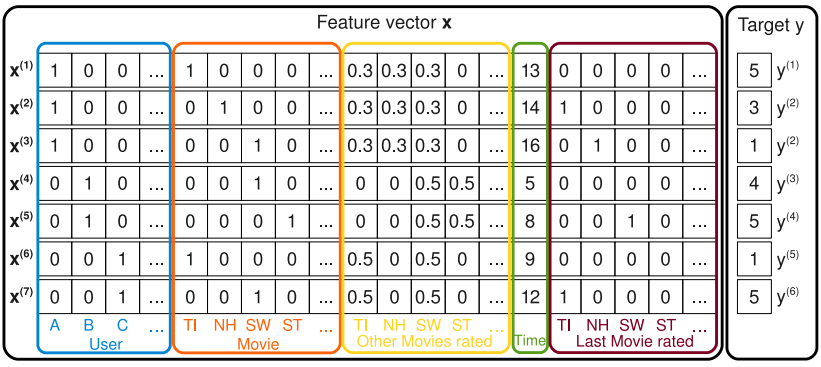
\includegraphics[width=0.8\textwidth]{rendle-ej.png}
\caption{Así es como quedaría la matriz del ejemplo con la estructura de datos descrita. En azul vemos la primeras $n$ columnas que corresponden a los usuarios, en naranja las $m$ columnas que corresponden a las películas, en amarillo nuevamente $m$ columnas que representan todos los items evaluados por el usuario de dicha observación. Por ultimo en verde la codificación temporal de la observación y el ultimo grupo, en marrón, representa la anterior película vista antes de la película activa correspondiente a dicho vector.}\label{fig:fm-ejemplo-full}
\end{figure}

Entonces la matriz del modelo quedaría como figura en el recuadro \ref{fig:fm-ejemplo-full}. En este caso consideramos como variables adicionales no solo el tiempo en el cual se evaluó la película, sino que también tomamos en cuenta el orden y el resto de películas evaluadas. En el caso del tiempo lo hemos codificado en meses desde Enero del 2009, aunque hay muchas otras formas de codificarlo. Por ejemplo miremos la segunda fila de las variables $x^{(2)}$, Alicia califico a Nothing Hill con 3 puntos 14 meses después de la fecha de referencia, es decir, en Febrero del 2010, habiendo solo evaluado hasta ese momento Titanic. Como solo poseemos tres observaciones para Alicia, esta observación representa el 33\% del total, entonces en amarillo representamos las tres películas que ha calificado (Titanic, Nothing Hill y Star Wars) y redondeamos dicho valor a 0.3 para cada una de la observaciones.
\hfill$\square$
\end{ejemplo}

%%%%%%%%%%%%%%%%%%%%%%%%%%%%%%%%%%%%%%%%%%%%%%%%%%%%
\subsection{Relación con regresión polinomial}

A primera vista el modelo propuesto de las máquinas de factorización de orden tiene una ecuación similar a un modelo de regresión polinomial de segundo grado (o una SVM con núcleo de orden 2):

\begin{equation}
\hat{y}^{(RP)}(x) = w_0 + \sum_{i=1}^{p} w_i x_i + \sum_{i=1}^{p} \sum_{j=1}^p w_{i,j} x_i x_j
\end{equation}

Donde los parámetros del modelo a estimar son:

\begin{equation*}
w_0 \in \mathbb{R}, \quad w \in \mathbb{R}^p, \quad \textbf{W} \in \mathbb{R}^{p \times p}
\end{equation*}

Si comparamos este modelo con el modelo que describimos en la ecuación \eqref{fm-orden2}, la diferencia que surge entre ellos es la forma de parametrizar las interacciones $w_{i,j}$. Para las regresión cuadrática estas interacciones son a priori independientes, mientas que en las FM asumimos que estas interacciones se pueden factorizar de la forma $\prodint{v_i,v_j}$, ya que supusimos que la matriz de datos es de bajo rango($w_{i,j}\approx \prodint{v_i,v_j}$). Por ejemplo, para un modelo de regresión clásico no existe una relación a priori entre dos interacciones $w_{i,j}$ y $w_{i,t}$, mientras que en las FM, al poder factorizar ambas como $\prodint{v_i,v_j}$ y $\prodint{v_i,v_t}$ respectivamente, existirá una dependencia que estará dada por $v_i$. De esta manera las FM, logran estimar las interacciones $w_{i,j}$ para pares (i,j) aunque existan pocas o ninguna interacción en los datos\cite{rendle2012factorization}. 

Como resultado de esta suposición, las FM tiene como ventaja tener que estimar menos parámetros, en la regresión polinomial estaremos estimando $\textbf{W} \in \mathbb{R}^{p \times p}$ por cual el orden de parámetros estará en el de $O(p^2)$. Mientras que las FM tendrán que estimar $O(pk)$ parámetros, que son muchos menos ya que $k$ es la cantidad de factores latentes que estamos suponiendo que tiene $\textbf{W}$.

%%%%%%%%%%%%%%%%%%%%%%%%%%%%%%%%%%%%%%%%%%%%%%%%
\section{Cálculo del modelo}

De forma similar a lo que hemos planteado para SVD, para calcular el modelo queremos considerar una función de pérdida a minimizar. En este caso consideraremos la función de pérdida cuadrática:

\begin{equation}
l(y,\hat{y}) = \norm{y-\hat{y}}_2	
\end{equation}

Introduciremos nuevamente un término de regularización dado por $\lambda >0$ para evitar que nuestro modelo sobreajuste a los datos, resultando de esta manera la función de perdida a optimizar:

\begin{equation}
\label{FMlossreg}
\sum_{i=1}^{T} l(y_i,\hat{y}(x_i)) + \frac{\lambda}{2} (\norm{w}^2 + \norm{\textbf{W}}^2)
\end{equation}

Para calcular los parámetros del modelo, podemos utilizar el descenso estocástico por gradiente o algún otro algoritmo de minimización. Para esto necesitamos calcular el gradiente de una FM de grado 2:

\begin{equation}
\frac{\partial}{\partial \theta} \hat{y}(x) =
\begin{cases}
1, &\text{si } \theta=w_0 \\
x_i, &\text{si } \theta=w_i \\
x_i (\sum_{j=1}^p v_{js} x_j) - v_{is}x_i^2, &\text{si } \theta=v_{is}
\end{cases}
\end{equation}

Entonces si llamamos $e(x) = y(x) - \hat{y}(x)$ los pasos de actualización del SGD estarán dados por:

\begin{equation}
\theta \leftarrow \theta(1-\alpha \lambda) + \alpha \cdot e(x) \cdot \frac{\partial}{\partial \theta} \hat{y}(x)
\end{equation}

Donde $\alpha>0$ es la tasa de aprendizaje, que determina la longitud de paso del algoritmo. 

La complejidad del modelo se encuentra en $O(kp^2)$, donde $p$ representa la cantidad de variables y $k$ es la dimensión de la factorización. Sin embargo veamos que puede computarse en orden lineal respecto a $k$ y a $p$ debido a la simetría del término cuadrático, es decir en $O(kp)$, para eso primero hagamos la siguiente observación:

\begin{lemma}
\label{fm-lema}
El cálculo de la ecuación \eqref{fm-orden2} se puede realizar en O(kp).
\end{lemma}

\begin{proof}
Consideremos la siguiente igualdad:

\begin{equation}
\label{eq:fm1}
\sum_{i=1}^p \sum_{j=1}^p \prodint{\mathbf{v}_i,\mathbf{v}_j} x_i x_j = \sum_{i=1}^p \sum_{j=i+1}^p \prodint{\mathbf{v}_i,\mathbf{v}_j} x_i x_j + \sum_{i=1}^p \sum_{j=1}^i \prodint{\mathbf{v}_i,\mathbf{v}_j} x_i x_j\\
\end{equation}

Si desarmamos el segundo término obtenemos que:

\begin{equation}
\label{eq:fm2}
\sum_{i=1}^p \sum_{j=1}^{i} \prodint{\mathbf{v}_i,\mathbf{v}_j} x_i x_j = \sum_{i=1}^p \sum_{j=1}^{i-1} \prodint{\mathbf{v}_i,\mathbf{v}_j} x_i x_j + \sum_{i=1}^p \prodint{\mathbf{v}_i,\mathbf{v}_i} x_i x_i
\end{equation}

Podemos hacer un cambio de indices en el primer término de la sumatoria $j=i-1 \Rightarrow i=j+1$, y nos queda que:

\begin{equation}
\label{eq:fm3}
\sum_{i=1}^p \sum_{j=1}^{i-1} \prodint{\mathbf{v}_i,\mathbf{v}_j} x_i x_j = \sum_{j=1}^p \sum_{i=j+1}^{p} \prodint{\mathbf{v}_j,\mathbf{v}_i} x_j x_i = \sum_{i=1}^p \sum_{j=i+1}^p \prodint{\mathbf{v}_i,\mathbf{v}_j} x_i x_j 
\end{equation}

Reemplazando \eqref{eq:fm2} y \eqref{eq:fm3} en \eqref{eq:fm1} y despejando obtenemos:

\begin{align}
\sum_{i=1}^p \sum_{j=i+1}^p \prodint{\mathbf{v}_i,\mathbf{v}_j} x_i x_j & = \frac{1}{2} \sum_{i=1}^p \sum_{j=1}^p \prodint{\mathbf{v}_i,\mathbf{v}_j} x_i x_j - \frac{1}{2} \sum_{i=1}^p \prodint{\mathbf{v}_i,\mathbf{v}_i} x_i x_i\\
& = \frac{1}{2} \big( \sum_{i=1}^p \sum_{j=1}^p \sum_{s=1}^k v_{is} v_{js} x_{i} x_j -\sum_{i=1}^p  \sum_{s=1}^k v_{is}^2 x_i^2 \big)\\
& = \frac{1}{2} \sum_{s=1}^k \big( \big( \sum_{i=1}^p v_{is} x_i \big) \big( \sum_{j=1}^p v_{js} x_j \big) - \sum_{i=1}^p  v_{is}^2 x_i^2 \big)\\
& = \frac{1}{2} \sum_{s=1}^k \big( \big( \sum_{i=1}^p v_{is} x_i \big)^2 - \sum_{i=1}^p  v_{is}^2 x_i^2 \big)
\end{align}

El término final tiene complejidad del orden de $O(kp)$.
\end{proof}

Entonces, gracias al lema \ref{fm-lema} si $x\in\mathbb{R}^p$ podemos reescribir a $\hat{y}$  como:

\begin{equation}
\hat{y}(x)=w_0+\sum_{i=1}^p w_i x_i + \frac{1}{2} \big[\sum_{s=1}^k \big( \big( \sum_{i=1}^p v_{is} x_i \big)^2 - \sum_{i=1}^p  v_{is}^2 x_i^2 \big) \big]
\end{equation}

Si para cada $s=1,\ldots,k$ calculamos previamente en cada paso el valor de $\sum_{i=1}^p v_{is} x_i$, podemos calcular el valor del gradiente en tiempo constante. Entonces para cada iteración que haga SGD sobre el conjunto de entrenamiento $E$, la complejidad será de $O(kp)$. 

%----------------------------------------------------------------------------------------
%   CAPITULO 3 
%----------------------------------------------------------------------------------------

\chapter{El problema del arranque en frío}

\section{Estableciendo el problema}

Cuando un usuario (o un ítem) ingresa por primera vez al sistema, el mismo no posee ninguna información referente a sus intereses. Debido a esto, un sistema basado en filtros colaborativos, no puede presentar items al usuario que sean de su preferencia. Esta, es una de las mayores dificultades en los sistemas de recomendación y es lo que se conoce como el problema del arranque en frío o $cold$-$start$\footnote{También se suele utilizar el término de Cold-Start para los casos de items (Cold ítem) o usuarios (Cold User) para los cuales se conocen muy pocos ratings.}.

Existen dos formas clásicas del problema de arranque en frío:

\begin{description}
\item[Usuario Nuevo] Un nuevo usuario ingresa al sistema por primera vez, para el cual no tenemos ningún historial de evaluaciones previas sobre los items del sistema.
\item[ítem Nuevo] Un nuevo ítem es agregado al sistema, por ejemplo en un sistema de recomendación de libros podría tratarse de un nuevo lanzamiento o en el caso de películas, una película estreno. Al igual que en el caso del usuario, al ser nuevo el ítem ningún usuario lo ha evaluado, por lo tanto no poseemos ratings previos en el historial del sistema que nos permita recomendarlo.
\end{description}

Bajo cualquiera de estos escenarios, el filtrado colaborativo puro, es decir sin información contextual, en general, no puede conseguir resultados robustos sobre la interacción entre los usuarios y los items, ya que no hay información disponible sobre la preferencia del usuario que sirva de base para las recomendaciones. En esta tesis nos centraremos en el problema de arranque en frío para un nuevo usuario, que de ahora en adelante llamaremos el problema del nuevo usuario por simplificación.

Existen múltiples acercamientos al problema, por ejemplo las técnicas basadas en contenido puede ayudar a cerrar la brecha de usuarios(o items) existentes a nuevos usuarios(o items), al inferir similitudes entre ellos a partir de características de los usuarios(items) como puede ser información contextual o información geográfica\cite{CS:schein2002methandmetrics}\cite{CS:New-son2016dealing}. Por lo tanto, pueden hacer recomendaciones para usuarios nuevos que tienen características similares a las de otros usuarios para los cuales si conocemos su comportamiento. También es usual encontrar sistemas que utilizan técnicas basadas en conocimiento, es decir que recurren a la interacción con el usuario, pidiendo que evalúe un cierto conjunto de items como parte del registro en el mismo sistema, por ejemplo un sistema que utiliza esta modalidad es el de Netflix o el de MovieLens\footnote{https://movielens.org/}\cite{CS:rashid2002getting}.

%Si bien los métodos basados en el contenido y basados en el conocimiento son más sólidos que los modelos colaborativos en presencia de inicios fríos, tal contenido o conocimiento puede no estar siempre disponible. Por lo tanto, se han diseñado varios métodos específicos para mejorar el problema del arranque en frío en el contexto de los sistemas de recomendación.

%%%%%%%%%%%%%%%%%%%%%%%%%%%%%%%%%
\section{Modelado del usuario vía entrevista}

Uno de los métodos mas populares para el tratar el problema del nuevo usuario es el de utilizar una entrevista con el usuario antes de que comience efectivamente a utilizar el sistema. En esta entrevista, le iremos presentando items para que el usuario evalúe y así poder ir recolectando información acerca de sus preferencias que podremos utilizar en nuestro modelo. La principal de las razones de la popularidad de esta metodología se debe a que no es computacionalmente costosa, y a la vez podremos utilizar las verdaderas preferencias del usuario, para poder predecir su comportamiento en general. Sin embargo, este escenario trae consigo dos principales cuestiones que son críticas, primero, como elegir los items para presentar al usuario, y segundo, que cantidad de items le requeriremos al usuario que evalue antes de terminar la entrevista.

Para responder estas cuestiones, tenemos que tener en cuenta dos aspectos. Para empezar, los items que vayamos a presentar tienen que tener un cierto valor "informativo" en el siguiente sentido, si presentamos un ítem que no posee valoraciones negativas del todo o viceversa, esto es, un ítem sobre el que haya un consenso, preguntarle al usuario acerca de dicho ítem puede carecer de importancia. Por ejemplo, en un sistema de recomendación de películas, preguntar por un "clásico" como Volver al Futuro(1985)\footnote{Según Google, a más del 95\% de los usuarios de Google les gustó Volver al Futuro} puede no ser tan informativo como preguntar por otra película que tenga mas variabilidad en sus ratings. 

Por otro lado, hay que también considerar la dificultad del proceso de entrevista, ya que si es muy costoso para el usuario, léase muchos items para evaluar, el usuario no utilizará el sistema o abandonará la entrevista en el transcurso de la misma\cite{CS:rashid2002getting}. Los motivos por los cuales una entrevista puede prolongarse demasiado, es que los items que le son presentados al usuario para evaluar no fueron vistos por el mismo. Esto, motiva a tener en cuenta la popularidad de los items a presentar, bajo la premisa de que mientras más popular sea un ítem, mas probables es que nuestro nuevo usuario la haya visto. Entonces, ya no solo es importante el rendimiento en la predicción que pueda hacer el sistema de los gustos de un usuario sino que también tendremos que tener presente el esfuerzo del usuario.

%%%%%%%%%%%%%%%%%%%%%%%%%%%%%%
\subsection{Selección no personalizada}\label{entrevistas}

La selección de items no personalizada, simplemente establece que para cada usuario le mostraremos los mismos items sin utilizar ninguna otra información personal.

\subsubsection{Popularidad}

Utilizando la información de la cantidad de valoraciones que tiene cada ítem en el sistema, clasificaremos a los items en forma descendente desde el más visto hasta el menos visto. Una vez hecho esto, iremos presentando los items en orden de popularidad hasta cumplir con la cuota de items a evaluar.

\textbf{Observación:} Es claro, que esta estrategia tiene como principal motivador lograr que el usuario consiga calificar rápidamente la cantidad preestablecida de items que pediremos evaluar. Sin embargo, a priori, podría sufrir del problema mencionado anteriormente de que los items presentados no sean informativos. Por otro lado, es posible que al preguntar por los items más populares, estemos agregando un gran sesgo. Esto es decir, los items que son mas populares, son los más fáciles de recomendar ya que poseen una gran cantidad de evaluaciones. Mientras que los items que tienen pocas evaluaciones sufren exactamente lo contrario, ya que una mala evaluación tendrá mayor peso para un ítem con pocas evaluaciones que uno popular\cite{CS:rashid2002getting}.

\subsubsection{Entropía}

La entropía es una medida utilizada para medir el contenido de información teórico que posee un ítem\cite{CS:kantor1986maxentropy}\cite{CS:rashid2008learning}. La entropía de un ítem $i$ la definimos de la siguiente forma:

\begin{equation}
Ent(i)=\sum_{r\in\mathcal{R}}P(r_i=r)\cdot \log(P(r_i=r))
\end{equation}

Donde $P(r_i=r)$ es la proporción de valoraciones $r$ que tuvo el ítem $i$ sobre todas las valoraciones que recibió. Mientras más grande sea la entropía de un ítem, mayor será el contenido potencial de información\cite{CS:rashid2002getting}.

Luego de calcular esto cada ítem, ordenamos en forma descendente los items para presentárselos al usuario por el valor de su entropía, ya que a mayor entropía, mayor es el supuesto contenido teórico del dicho ítem.

\textbf{Observación:} El acercamiento por entropía supone dos dificultades que no son claras de manejar. La primera es que hacer con los valores faltantes de evaluaciones del ítem que sabemos que se deben a múltiples factores. Segundo, ordenar por entropía supone que tenemos en cierta forma que el ítem es más informativo, pero por ejemplo, un ítem con dos o tres ratings diferentes puede tener mayor entropía, que uno con muchos mas ratings pero menos distribuidos. De esta manera, mas informativo no va a condecir necesariamente con más útil al sistema.

\subsubsection{Estrategia Balanceada}

Como se comento anteriormente, la entropía pura puede terminar preguntando por items que muy poca gente ha visto por lo cual es difícil que el usuario nuevo pueda evaluarlo, y la popularidad puede no ser informativa. Es decir que estas dos características no parecen ser dependientes una de la otra\cite{CS:rashid2002getting}. Esto nos motiva a considerar la siguiente medida propuesta en Rashid et al\cite{CS:rashid2002getting} para ordenar los items a presentar:

\begin{equation}
\label{eq:bal}
LogPopEn(i) = \log(Pop(i))\cdot Ent(i)
\end{equation}

Una vez calculada esta medida, se ordena de manera descendente los items según este valor obtenido y se los presentaremos al usuario.

\textbf{Observación:}  Como dijimos anteriormente, existe un intercambio y posible independencia entre la entropía y la popularidad, lo cual esta estrategia balanceada apunta a capturar. Podríamos considerar también no utilizar el logaritmo en la popularidad pero en general la popularidad es varias magnitudes mayor a la entropía, por lo cual dominaría completamente nuestra medida sobre los items.

\subsubsection{Aleatoria}

En la selección aleatoria, presentaremos los items con probabilidad uniforme  sobre todos los items que posee el sistema. Esta estrategia la utilizaremos para poder comparar de los otros métodos. 

%%%%%%%%%%%%%%%%%%%%%%%%%%%%%%
\subsection{Selección personalizada}

En la selección personalizada, el objetivo es que cada valoración que el usuario aporte sobre un ítem sea utilizada para seleccionar el/los próximos items a presentarle para evaluar. 

\subsubsection{Selección ítem-ítem}

En esta estrategia\cite{CS:rashid2002getting}, presentaremos items con alguna de las estrategias antes enunciadas hasta que el usuario evalue un ítem que conoce. Una vez evaluado ese ítem, calculamos su similitud con otros items y comenzamos a presentarle items que se encuentran en la vecindad de los que ya ha evaluado. A medida que el usuario logra evaluar mas items, vamos actualizando la lista, sin repetir los items que ya hemos mostrado.

\textbf{Observación:} Esta técnica apunta nuevamente a encontrar de manera rápida items que el usuario pueda evaluar, actualizando los items a mostrar gracias a los ratings que el usuario ha proveído. Sin embargo, existe una posible desventaja, al mostrar al usuario, items similares a los que ya ha evaluado, puede suceder que el sistema muestre items demasiado correlacionados entre sí. Por ejemplo, en un sistema de recomendación de películas, si el usuario ya ha evaluado a \textit{Star Wars}-Episodio IV(1977), ya sea positivamente o no, es altamente probable que \textit{Star Wars}-Episodio V(1980) u otra película de la saga, pertenezca a la vecindad de la misma y que el usuario tenga la misma preferencia por dicha película. De esta manera, colectaríamos demasiadas películas que le gusten o demasiadas películas que no le gusten al usuario.


%%%%%%%%%%%%%%%%%%%%%%%%%%%%%%%%%%%%%%%%
\section{Alternativas} \label{cap:propuestas}

El proceso de entrevistas, posee dos grandes desventajas:

\begin{itemize}
\item \textbf{Re-entrenamiento}: Para poder realizar recomendaciones a los usuarios, utilizamos los resultados de las entrevistas para re-entrenar el modelo y poder realizar predicciones con el nuevo modelo. Realizar esto no resulta escalable para grandes sistemas de recomendación 
\item \textbf{Dificultad para el Usuario}: Aunque el objetivo de las diferentes formas de seleccionar los items es también el de minimizar la el esfuerzo que le requiere al usuario poder evaluar items, puede que esto no sea algo que el usuario este dispuesto a realizar, lo cual podría hacer que desista de utilizar el sistema.
\end{itemize}

Bajo estas dificultades existen múltiples enfoques que utilizan variables de contexto relacionadas al usuario y a los items para poder realizar recomendación sin utilizar las entrevistas\cite{CS:New-son2016dealing}. De esta forma evitamos ambos problemas pero a costo de perder precisión en las predicciones.

\subsubsection{Propuesta}

En este contexto, propondremos una forma diferente de modelar un usuario, inspirados en la técnica de vecinos más cercanos y aprovechando las facilidades y versatilidad que otorgan las máquinas de factorización para involucrar este tipo de información. Para esto lo que haremos sera construir un vector $x$ de variables, utilizando su información contextual y sus vecinos en un sentido similar al de kNN.

Formalmente, supongamos que $u$ es un usuario nuevo que ingresa a un sistema ya entrado con una máquina de factorización que utiliza información contextual del usuario como lo descrito en la sección \ref{context}. Supondremos que esta información relacionada a las características del usuario(edad, sexo, profesión, dirección, ingresos, etc.) la podemos cuantificar de alguna forma en un vector $f(u)\in \mathbb{R}^d$, donde $d$ es la cantidad de características a las que tenemos acceso ya pre-procesado. Por ejemplo, si poseemos la profesión podemos asignarles etiquetas numéricas, o si se trata de la dirección podemos codificarlo con etiquetas de provincias, o regiones.

Nuestro modelo entrenado de FM esta dado por la función de ratings $\hat{y}(x):\mathbb{R}^p \rightarrow \mathcal{R}$, donde $p=n+m+d$. Entonces, si quisiéramos, podemos utilizar $\hat{y}$ para predecir la valoración sobre un ítem $j$ para este usuario, donde el vector $x^{(u,j)}\in\mathbb{R}^{p}$ es:

\begin{equation}\label{eq:m1-base}
x^{(u,j)} = ( \underbrace{0,\ldots,0}_{\substack{\text{Usuario}}}, \underbrace{0,\ldots,0,1,0,\ldots,0}_{\substack{\text{j-ésimo ítem}}},  \underbrace{f_1,\ldots,f_d}_{\substack{\text{f(u)}}})
\end{equation}

Las primeras $n$ posiciones, tendría solo ceros ya que no se encuentra en el sistema, las siguientes $m$ posiciones codifican el ítem y las ultimas $d$ posiciones caracterizan las variables del usuario. Las únicas interacciones que tendría $\hat{y}(x^{(u,j)})$ serían con el mismo ítem y los usuarios de iguales características, por lo que podríamos estar perdiendo mucha expresividad del modelo, que quedaría:

\begin{equation}
\label{eq:prop0}
\hat{y}(x^{(u,j)}) = w_0+ w_j + \sum_{s = 1}^d w_s f_s + \sum_{s=1}^d \sum_{s'>s}^d \prodint{\mathbf{v}_s,\mathbf{v}_t} f_s f_{s}
\end{equation}

Donde  $w_0 \in \mathbb{R}, \quad w \in \mathbb{R}^p, \quad \textbf{V} \in \mathbb{R}^{p \times {q}}$. Notar el pequeño abuso de notación que hicimos en $\sum_{s = 1}^d w_s f_s$ donde $w_s$ representan a las coordenadas de $w$ que corresponden a las $f_s$, es decir que en realidad $w_s$ es un $w_{j_s}$ con $j_s = p-s+1, \ldots, p$. Realizamos el mismo abuso en los $\textbf{V}_s$.

Lo que propondremos entonces, es construir un vector $x$ para representar al usuario nuevo, utilizando los usuarios que más se parezcan a el, con respecto a sus variables demográficas. De esta forma estamos recurriendo a la misma lógica que describimos con kNN, esto es, asumir que usuarios con características personales similares, tendrán similares preferencias sobre los items. 

Consideremos $N_k(u)$ el conjunto de los $k$ usuarios más cercanos (según alguna métrica) al usuario $u$ dentro del conjunto del conjunto de entrenamiento $E$. Entonces pensaremos al usuario $u$ como una combinación de sus vecinos en $N_k(u)$. Lo que haremos es mirar las primeras $n$ coordenadas(las correspondientes a los usuarios) estarán dadas por:

\begin{equation}
\label{prop1}
\bar{x}_v^{(u,j)}=
\begin{cases}
1/k &\text{si } v\in N_k(u) \\
0 &\text{caso contrario}
\end{cases}
\end{equation}

Entonces el vector que utilizaremos será:

\begin{equation}
x^{(u,j)} = ( \underbrace{\bar{x}^{(u,j)}}_{\substack{\text{Usuario}}}, \underbrace{0,\ldots,0,1,0,\ldots,0}_{\substack{\text{j-ésimo ítem}}},  \underbrace{f_1,\ldots,f_d}_{\substack{\text{f(u)}}})
\end{equation}

De esta forma, la predicción para este usuario quedará de la siguiente forma:

\begin{equation}
\label{eq:prop1}
\begin{split}
\hat{y}(x^{(u,j)}) = w_0+ w_j + \frac{1}{k} \sum_{v\in N_k(u)} w_v & + \sum_{s = 1}^d w_s f_s + \sum_{s=1}^d \sum_{s'>s}^d \prodint{\mathbf{v}_s,\mathbf{v}_t} f_s f_{s} \\
& + \frac{1}{k^2}\sum_{v\in N_k(u)} \sum_{v'\in N_k(u): v'>v} \prodint{\mathbf{v}_v,\mathbf{v}_{v'}} 
\end{split}
\end{equation}

Si comparamos ambas predicciones, \eqref{eq:prop0} y \eqref{eq:prop1} vemos que aparecen ahora dos términos extras que involucran la relación con los vecinos del usuario $u$ pesadas sobre la cantidad de vecinos que hemos considerado. Esta aproximación, al involucrar más interacciones entre las variables, tiene la posibilidad de mejorar la expresividad del modelo en este contexto de arranque en frío.

Una segunda propuesta que también hemos, de manera exactamente análoga a lo recién descrito, es cambiar la forma en la que pesamos los usuarios vecinos del usuario activo. En vez de pesarlos de manera idéntica, lo que haremos será considerar los inversos de  las distancias mas algún parámetro de contracción $\beta \geq 1$, de esta forma el vector de variables quedaría codificado para los usuarios como: 

\begin{equation}
\label{prop2}
\bar{x}_v^{(u,j)}=
\begin{cases}
\frac{1}{d(u,v)+\beta} &\text{si } v\in N_k(u) \\
0 &\text{caso contrario}
\end{cases}
\end{equation}

Al hacer esto lo que logramos, es darle mayor importancia al usuario más similar a $u$ y quitarles peso a los usuarios que no sean tan parecidos. En este caso la predicción quedaría muy similar a \eqref{eq:prop1} pero en vez de tener los pesos de $\frac{1}{k}$ fuera de las sumatorias, aparecerían los inversos de las distancias dentro de las sumas.

El término de contracción que utilizaremos será $\beta = \sqrt{k}$ lo incluimos para evitar dividir por cero. Pero también nos sirve en el caso de que por ejemplo el usuario tenga muchos usuarios que se encuentran a distancia 0 ya que en ese caso los términos que involucran a los usuarios quedarían sumados entre sí, sin realizar un promedio, lo cual nos llevaría a predicciones erróneas.

Las distancias que consideraremos entre $u$ y $v$ será la norma $\norm{.}_1$ de la diferencia entre los vectores de variables de usuarios $f(u)$:

\begin{equation}
\label{eq:manhattan}
d(u,v) = \norm{f(u)-f(v)}_1 = \sum_{j=1}^d \abs{f(u)_j-f(v)_j}
\end{equation}

%%%%%%%%%%%%%%%%%%%%%%%%%%%%%%%%%%%%%%%%%%%%%%%%%%%%%%%%%%%%
%%%%%%%%%%%%%%%%%%%%%%%%%%%%%%%%%%%%%%%%%%%%%%%%%%%%%%%%%%%%
%%%%%%%%%%%%%%%%%%%%%%%%%%%%%%%%%%%%%%%%%%%%%%%%%%%%%%%%%%%%
\chapter{Simulaciones}

En este capítulo expondremos los procedimientos llevados a cabo para comparar los rendimientos en los distintos escenarios de las máquinas de factorización de orden 2 frente a las técnicas clásicas kNN basada en items utilizando la similitud coseno y la similitud pearson, Slope One y SVD.

\section{Datos}

Para los experimentos utilizaremos el conjunto de datos de \textit{MovieLens-100k}\cite{harper2016movielens} de ratings de un sistema de recomendación de películas implementado por el grupo de investigación \textit{GroupLens} de la Universidad de Minnesota. Este conjunto de datos contiene 100000 ratings del 1 al 5 que dieron 943 usuarios sobre 1642 películas, en el cual cada usuario evaluó al menos 20 películas. Además también nos proporciona datos básicos sobre los usuarios: edad, sexo, profesión(un total de 21 profesiones) y un código postal de EEUU. Sobre los items nos proporciona varios datos que incluyen género(19 géneros posibles), fecha de estreno y fecha de lanzamiento de la versión compacta.

\begin{figure}[!ht]
\centering
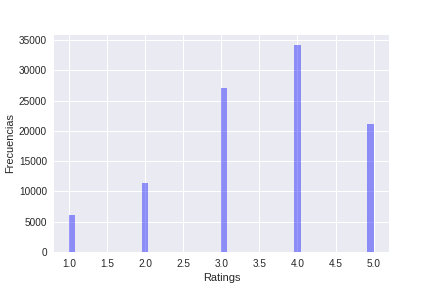
\includegraphics[width=0.8\textwidth]{graficos/frecratings.png}
\caption{Distribución de ratings de MovieLens.}\label{fig:frec-rat}
\end{figure}

\subsubsection{Preprocesamiento para FM}

Los datos de contexto que utilizamos para las máquinas de factorización tuvieron que ser procesados para tener la estructura que necesitamos. Las variables del usuario que consideramos fueron:

\begin{itemize}
\item \textbf{Edad} La edad la categorizamos por rangos $[a_i,a_{i+1})$ con $i= 1,\ldots,9$ y con eso construimos un vector $edad(u)\in \mathbb{R}^9$ de tal forma que $edad(u)_i$ = 1 si y solo si $edad(u)_i \in [a_i,a_{i+1})$. En este caso los intervalos para las edades fueron predefinidos. En el gráfico \ref{fig:edades} podemos observar la distribución de las edades.
\item \textbf{Sexo} El sexo lo categorizamos como dos variables binarias masculino y femenino.
\item \textbf{Profesión} La profesión la codificamos en un vector binario de longitud 21 (que es la cantidad de profesiones que admite el sistema), donde la i-ésima posición es 1 solo si corresponde a la profesión del usuario. De lo contrario esa posición es 0.
\end{itemize}

En el caso de los items, la única variable que utilizamos fue el género de la película, que lo codificamos de las misma manera que hicimos con las profesiones, pero esta vez, el vector tendrá longitud 19. Notaremos $f(u)$ al vector que representa todas la variables del usuario y $f(i)$ a las del ítem, en nuestro caso solo los géneros.

\begin{figure}[!ht]
\centering
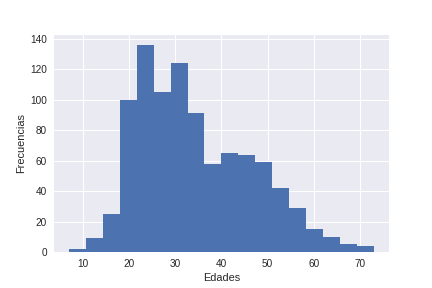
\includegraphics[width=0.8\textwidth]{graficos/edades.png}
\caption{Distribución de las edades}\label{fig:edades}
\end{figure}

\section{Implementación}

Para realizar las simulaciones y experimentos con todas les técnicas descritas en el capitulo uno, utilizamos el paquete para sistemas de recomendación Surprise\cite{Surprise} implementado sobre la librería SciPy\footnote{https://www.scipy.org} de Python. Además también utilizamos la librería Scikit-learn\footnote{http://scikit-learn.org/stable/}, una popular librería de aprendizaje automático implementada en Python. 

Para las máquinas de factorización existen varias implementaciones en Python, por ejemplo FastFM\cite{fastfm} y LightFM\cite{lightfm} son dos de ellas, también contamos con la implementación LibFM en C++\cite{rendle2012factorization} del propio Rendle. Todas ellas implementan varias funciones de pérdida además de pérdida cuadrática considerada y varios optimizadores además de SGD. Elegimos utilizar una implementación de propósito académico llamada TFFM\cite{tffm2016}, basada en TensorFlow\footnote{https://www.tensorflow.org/}. Dentro de esta implementación, utilizamos como optimizador el algoritmo basado en gradiente de primer orden $Adam$\cite{kingma2014adam}.

\section{Simulación 1 - Recomendación}

El objetivo de este primer experimento es ver como se comportan las máquinas de factorización frente a las técnicas clásicas descritas en el capitulo uno, en los problemas clásicos de predicción y recomendación. 

Para las máquinas de factorización consideramos tres conjuntos diferentes de variables que nos determinarán tres máquinas diferentes de factorización. Estos conjuntos fueron:

\begin{itemize}
\item \textbf{FM-Us}: Las variables utilizadas fueron (Usuario(u), Pelicula(i), f(u))
\item \textbf{FM-It}: Las variables utilizadas fueron (Usuario(u), Pelicula(i), f(i))
\item \textbf{FM-All}: Las variables utilizadas fueron (Usuarios(u), Peliculas(i), f(u), f(i))
\end{itemize}

\subsubsection{Procedimiento}

Primero dividimos los datos de MovieLens en un conjunto de entrenamiento $E$ y un conjunto de testeo $T$, con 75000 y 25000 entradas respectivamente. Para los algoritmos SVD y FM usaremos los mismos parámetros como figuran en el cuadro \ref{tb:params1}.

\begin{table}[ht]
\centering
\begin{tabular}{|c|c c c c|}
\hline
Algoritmo & $\alpha$ & $\lambda$ & Factores & Epochs\\
\hline
SVD & 0.005 & 0.002 & k = 25 & 120 \\
FM & 0.005 & 0.002 & k = 25 & 120 \\
\hline
\end{tabular}
\caption{Parámetros utilizados por los algoritmos}
\label{tb:params1}
\end{table}

Donde $epochs$ representa la cantidad de iteraciones que realizaremos en los respectivos SGD, utilizándolo como criterio de parada para el algoritmo. Cabe mencionar que estamos utilizando el mismo valor de tasa de aprendizaje y de regularización para todas las variables, y no los distinguimos entre si. Mientras que para kNN utilizaremos como cantidad de vecinos $k=40$ como viene por defecto en la implementación de Surprise.

\subsubsection{Resultados - Predicción}

En el recuadro \ref{tb:resul1} reportamos los resultados obtenidos con los diferentes modelos propuestos, tanto para el RMSE como para el MAE, así como los tiempos de ejecución.

\begin{table}[h]
\centering
\begin{tabular}{|c|c c c|}
\hline
Algoritmo & RMSE & MAE & Tiempo \\
\hline
kNN - Coseno & 1.030688 & 0.815971 & 00:00:09.3\\
kNN - Pearson & 0.998876 & 0.787209 & 00:00:06.9 \\
Slope One & 0.948320 & 0.744437 & 00:00:04.2 \\
SVD & 0.923945 & \textbf{0.727080} & 00:00:14.9\\
FM-us & 0.898077 & 0.746818 & 0:00:21.9 \\
FM-it & 0.889801 & 0.741622 & 0:00:21.9\\
FM-all & \textbf{0.888645} & 0.7410826 & 0:00:21.9 \\
\hline
\end{tabular}
\caption{RMSE y MAE para las diferentes técnicas.}
\label{tb:resul1}
\end{table}

Se puede observar, como los modelos de máquinas de factorización tienen un rendimiento superior a las otras técnicas según el error cuadrático. Sin embargo, al observar el valor del MAE, notamos que las máquinas de factorización son superadas por SVD, y no muestran un rendimiento superior al obtenido por Slope One.

Por otro lado, se observa que los rendimientos entre los diferentes modelos de FM, no son significativamente diferentes en este experimento en comparación a la diferencia con el resto de las técnicas. Siendo así, \textbf{FM-all}, la que obtiene el mejor rendimiento de las tres por poco.

En cuanto a los tiempos de ejecución, era de esperar que sean menores los tiempos de kNN y de Slope One, debido a su simplicidad algorítmica, lo cual las permite ejecutar rápidamente. Mientras que SVD y los modelos de FM, tienen mayores tiempos de ejecución ya que se trata de modelos mas complejos. Aun así, a pesar de que los modelos de FM tienen diferentes tamaños, eso no termina impactando en los tiempos de ejecución.

\subsubsection{Resultados - Recomendación}

Para medir la recomendación, utilizaremos MAP@K descrita en \eqref{err:map} y NDCG@k descrita en \eqref{err:ndcg} para diferentes valores de k. En este experimento, solo consideraremos \textbf{FM-all}. Los resultados obtenidos para MAP se pueden apreciar en el gráfico \ref{fig:map} mientras que los obtenidos para NDCG pueden observarse en el gráfico \ref{fig:ndcg}.

En el problema de recomendación, las FM mostraron un rendimiento superior a kNN. Sin embargo no lograron traducir los buenos resultados de predicción en buenas recomendaciones como si lo hizo SVD. Las FM solo lograron tener un rendimiento similar al obtenido con Slope One.

\begin{figure}[!ht]
\centering
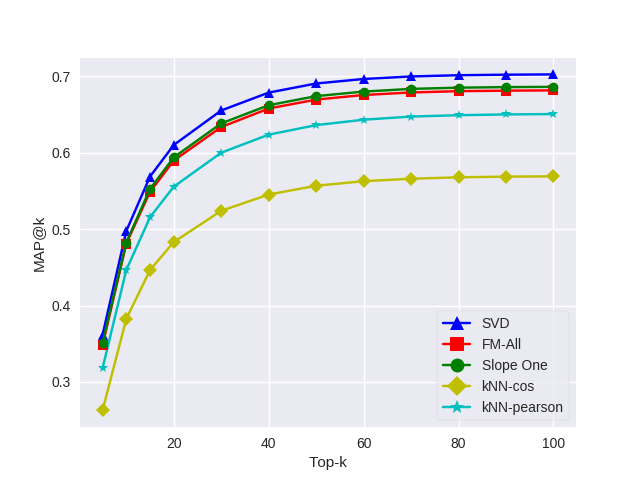
\includegraphics[width=0.8\textwidth]{graficos/map1.png}
\caption{Errores según MAP@k en el Top-k.}\label{fig:map}
\end{figure}

\begin{figure}[!ht]
\centering
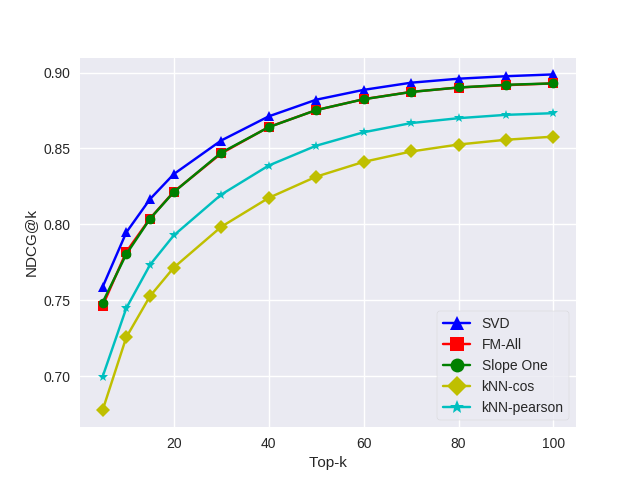
\includegraphics[width=0.8\textwidth]{graficos/ndcg1.png}
\caption{Errores según NDCG@k en el Top-k}\label{fig:ndcg}
\end{figure}

\section{Simulación 2 - Entrevistas}

El objetivo de esta simulación es la de analizar el rendimiento de las máquinas de factorización en el problema de arranque en frío, utilizando una estrategia de entrevistas para modelar el perfil del usuario como lo visto en el capítulo tres. De esta forma, podremos analizar si el modelo de \textbf{FM-all} logra mejorar la expresividad del sistema frente a SVD en un escenario de arranque en frío. Para esto, simularemos el funcionamiento de un sistema de recomendación como MovieLens, el cual le solicita a un usuario nuevo al ingresar por primera vez al sistema, que evalúe una determinada cantidad de items. En esta simulación elegimos emular el comportamiento de SVD con una máquina de factorización como fue descrito en \eqref{eq:fm-svd} para obtener resultados mas confiables.

\subsubsection{Procedimiento}

Para este escenario, dividimos el conjunto de datos $D$ entre conjunto de datos de entrenamiento $E$ y de testeo $T$ de forma disjunta en los usuarios, a los que notaremos como $E_{us}$ y $T_{us}$ respectivamente. Esto es para poder imitar el proceso del ingreso de un nuevo usuario en el sistema, por lo que $T_{us}\cap E_{us} = \emptyset$. Para esto seleccionamos de manera aleatoria a los usuarios para agregar a $T$, quitándolo de $D$ junto a todos sus ratings, manteniendo una proporción de entre el 20\% y el 25\% de datos en $T$. Las observaciones restantes contenidas en $D$, constituirán el conjunto de entrenamiento $E$.

\begin{figure}[ht]
\centering
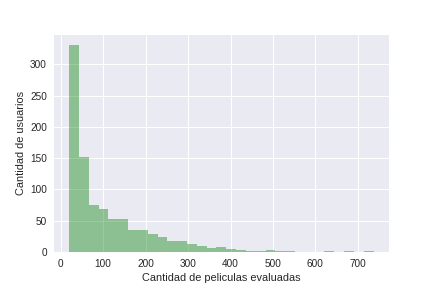
\includegraphics[width=0.9\textwidth]{graficos/pelis-usuarios.png}
\caption{Cantidad de peliculas que evaluaron los usuarios en el conjunto de datos}\label{fig:usu-cantpelis}
\end{figure}

La selección de usuarios para el arranque en frío, estuvo sujeta a que los usuarios hubiesen evaluado al menos 100 películas y menos de 200, siguiendo un procedimiento similar al realizado en Rashid et. al.\cite{CS:rashid2008learning}. Esto lo realizamos para asegurarnos poder solicitar al usuario que evalúen una cierta cantidad de items, ya que de lo contrario podría haber usuarios en $T_{us}$ que tienen menos observaciones que la cantidad de películas que le pedimos evaluar, emulando lo que haría un sistema de recomendación. El corte superior de 200 fue elegido para evitar perder usuarios en el conjunto de datos que sean muy significativos, ya que es poca la cantidad de usuarios que evaluaron muchas películas como se puede observar en \ref{fig:usu-cantpelis}. En esta simulación, de un total de 943 usuarios, 788 usuarios pertenecen a $E_{us}$ y 155 usuarios pertenecen a $T_{us}$.

Para presentar las películas para el nuevo usuario evalúe, elegimos la estrategia balanceada definida en \ref{entrevistas}, que mostró un rendimiento superior a las mencionadas en la precisión de la predicción \cite{CS:rashid2002getting}.Esta elección se debe a que el objetivo de esta simulación no es la de comparar las estrategias de selección de items, sino evaluar los rendimientos en las predicciones. Le presentamos películas hasta que logre evaluar $q$ de ellas, donde $q = 10,15,20,25$.

Finalmente compararemos los errores entre \textbf{FM-all} y SVD, utilizando los mismos parámetros que en la primer simulación \ref{tb:params1}, pero para diferentes cantidades de factores $f=15,25,50,100$ con el objetivo de analizar su impacto en el problema. Para calcular el error, utilizamos el RMSE y MAE, pero en vez de hacerlo sobre todo el conjunto de testeo $T$, lo hicimos sobre cada usuario en el conjunto $T_{us}$ y luego promediamos sobre los usuarios. Esto tiene sentido ya que queremos ver como es el rendimiento individual del sistema para el escenario de un nuevo usuario. 

El procedimiento realizado, se encuentra detallado en \ref{alg:entre}.

\begin{algorithm}[ht]
\begin{algorithmic}[ENTREVISTA]
%\REQUIRE Matriz de ratings $R$, learning rate $\alpha$, $\lambda$ 
%\ENSURE $b,p,q$
\FORALL {Usuario $u \in T_{us}$}
\WHILE {$u$ no haya evaluado $q$ películas}
\STATE Presentar la próxima película $i$
\IF {$u$ pudo evaluar $i$}
\STATE Agregar al usuario $u$ junto a $i$ y el rating provisto al conjunto $E$
\STATE Remover la observación de $T$
\ENDIF
\ENDWHILE
\STATE Entrenar modelo \textbf{M} con $\tilde{E}$
\STATE Calcular el error de predecir el resto de las películas de $u$ en $\tilde{T}$
\ENDFOR
\STATE Promediar los errores obtenidos para cada usuario en $T_{us}$
\end{algorithmic}
\caption{Procedimiento de entrevista}\label{alg:entre}
\end{algorithm}

\subsubsection{Resultados}

En la tabla \ref{tb:resul-base} se encuentran los errores obtenidos al calcular las predicciones directamente con el conjunto $E$, lo cual claramente tiene un mal rendimiento. Aun así, gracias a la información de contexto, el modelo \textbf{FM-all}, logra resultados que son mas razonables. Resulta interesante notar, que en este contexto, el aumento en la cantidad de factores, no mejora los resultados sino que los empeora para cualquiera de los dos modelos.

\begin{table}[ht]
\centering
\begin{tabular}{c|c|c c c c}
			& Errores & $f=15$ & $f=25$ & $f=50$ & $f=100$ \\
\hline
\multirow{2}{*}{SVD}& RMSE & 9.811 & 10.352 & 11.013 & 11.490 \\
					& MAE & 2.938 & 3.028 & 3.134 & 3.209 \\
\hline
\multirow{2}{*}{FM} & RMSE & 1.707 & 1.737 & 1.789 & 1.849 \\
					& MAE & 1.071 & 1.081 & 1.101 & 1.122\\
\end{tabular}
\caption{Errores según la cantidad de factores para SVD y \textbf{FM-all} sin encuestas}
\label{tb:resul-base}
\end{table}

En las figuras \ref{fig:entr1}, \ref{fig:entr2}, \ref{fig:entr3} y \ref{fig:entr4}, graficamos los errores (RMSE y MAE) en función de la cantidad de películas solicitadas $q$, para cada elección de factores. 

\begin{figure}[ht]
\centering
    \begin{subfigure}[b]{0.5\textwidth}            
            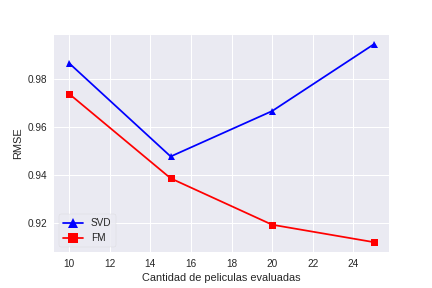
\includegraphics[width=\textwidth]{graficos/entr-15-rmse.png}
            %\label{fig:SRl}
    \end{subfigure}%
     %add desired spacing between images, e. g. ~, \quad, \qquad etc.
      %(or a blank line to force the subfigure onto a new line)
    \begin{subfigure}[b]{0.5\textwidth}
            \centering
            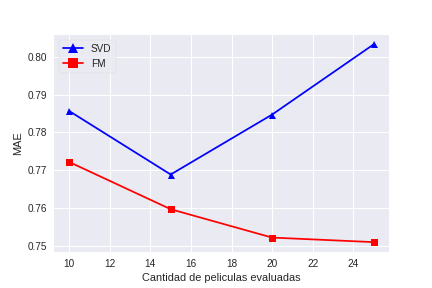
\includegraphics[width=\textwidth]{graficos/entr-15-mae.png}
            %\label{fig:SRl2}
    \end{subfigure}
    \caption{Errores con $f=15$}\label{fig:entr1}
\end{figure}

\begin{figure}[ht]
\centering
    \begin{subfigure}[b]{0.5\textwidth}            
            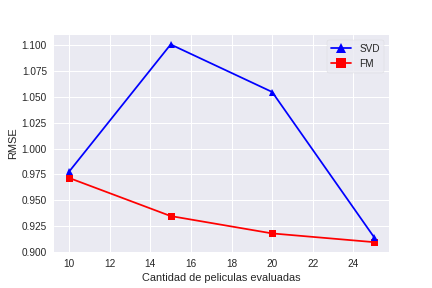
\includegraphics[width=\textwidth]{graficos/entr-25-rmse.png}
            %\label{fig:SRl}
    \end{subfigure}%
     %add desired spacing between images, e. g. ~, \quad, \qquad etc.
      %(or a blank line to force the subfigure onto a new line)
    \begin{subfigure}[b]{0.5\textwidth}
            \centering
            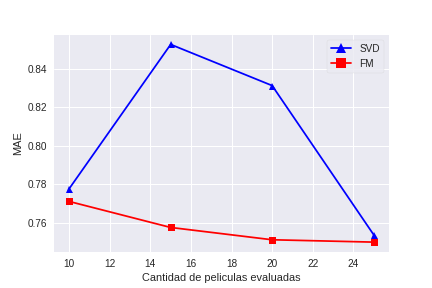
\includegraphics[width=\textwidth]{graficos/entr-25-mae.png}
            %\label{fig:SRl2}
    \end{subfigure}
    \caption{Errores con $f=25$}\label{fig:entr2}
\end{figure}

\begin{figure}[!ht]
\centering
    \begin{subfigure}[b]{0.5\textwidth}            
            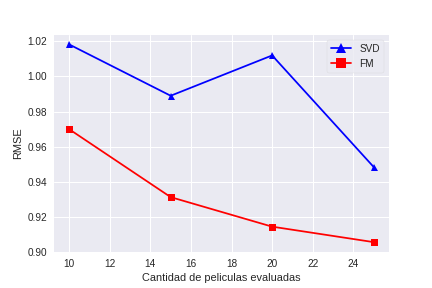
\includegraphics[width=\textwidth]{graficos/entr-50-rmse.png}
            %\label{fig:SRl}
    \end{subfigure}%
     %add desired spacing between images, e. g. ~, \quad, \qquad etc.
      %(or a blank line to force the subfigure onto a new line)
    \begin{subfigure}[b]{0.5\textwidth}
            \centering
            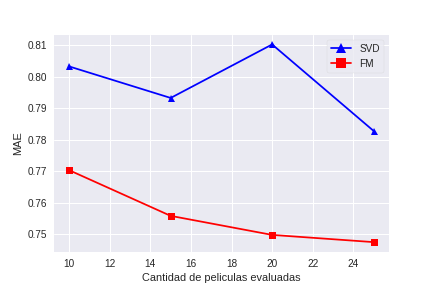
\includegraphics[width=\textwidth]{graficos/entr-50-mae.png}
            %\label{fig:SRl2}
    \end{subfigure}
    \caption{Errores con $f=50$}\label{fig:entr3}
\end{figure}

\begin{figure}[ht]
\centering
    \begin{subfigure}[b]{0.5\textwidth}            
            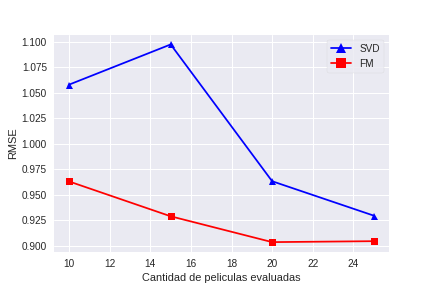
\includegraphics[width=\textwidth]{graficos/entr-100-rmse.png}
            %\label{fig:SRl}
    \end{subfigure}%
     %add desired spacing between images, e. g. ~, \quad, \qquad etc.
      %(or a blank line to force the subfigure onto a new line)
    \begin{subfigure}[b]{0.5\textwidth}
            \centering
            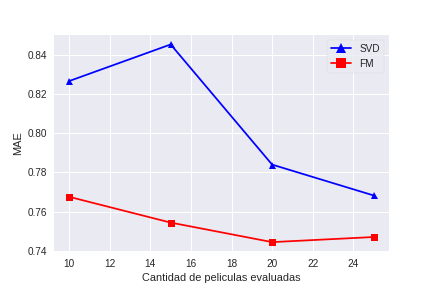
\includegraphics[width=\textwidth]{graficos/entr-100-mae.png}
            %\label{fig:SRl2}
    \end{subfigure}
    \caption{Errores con $f=100$}\label{fig:entr4}
\end{figure}

En todas ellas, el modelo de \textbf{FM-all} tiene un rendimiento superior que el modelo SVD en ambas métricas. En los casos donde consideramos pocos factores, es donde más se destacan esas diferencias de rendimiento a favor de \textbf{FM-all}. En el caso de 25 factores, SVD logra emparejar su rendimiento a FM al pedirle al usuario que evalué 10 películas, pero luego el error empeora al solicitar más ratings, volviendo a rendir de igual manera que FM al evaluar 25 películas. Este comportamiento con baja cantidad de factores, evidencia la dificultad que tiene el modelo clásico de SVD para predecir ratings en casos de pocos ratings. Aun así, no hay que descartar el efecto que pueden tener $\alpha$ y el parámetro de regularización en estos casos, por lo cual serían necesarias mas simulaciones para explicar con precisión este comportamiento.

En los casos donde consideramos 50 y 100 factores, el modelo de FM tiene un comportamiento superior a SVD con pocos ratings provistos por los usuarios(10 y 15), mostrando como el modelo propuesto tiene una expresividad superior a SVD, ya que con poca información provista por los usuarios, consigue mejores predicciones en promedio. Una vez que los usuarios proveen mas ratings, SVD empieza a mejorar su rendimiento pero aun por debajo del de FM.

En la figura \ref{fig:comp-fact} podemos ver una comparación de los diferentes modelos de FM considerados según la cantidad de factores. En todos ellos observamos como mejora el rendimiento a medida que los usuarios proveen mas ratings. El aumento en la cantidad de factores para la FM, se vio traducido en una mejora de los errores, pero cuando la cantidad de ratings provistos fueron pocos (10 y 15), esa mejora no es tan significativa como lo es cuando aumenta $q$. Esto evidencia que las FM pudieron obtener buenos resultados sin la necesidad de muchos ratings, lo cual nos vuelve a hablar de la expresividad de este modelo. Esto es una gran ventaja, ya que el entrenamiento de una FM con mayor cantidad de factores es más costoso computacionalmente pues que la complejidad depende de los mismos.

\begin{figure}[!ht]
\centering
    \begin{subfigure}[b]{0.5\textwidth}            
            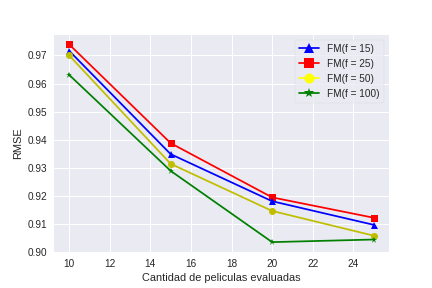
\includegraphics[width=\textwidth]{graficos/entr-factores-rmse.png}
            \caption{Errores RMSE}
            %\label{fig:SRl}
    \end{subfigure}%
     %add desired spacing between images, e. g. ~, \quad, \qquad etc.
      %(or a blank line to force the subfigure onto a new line)
    \begin{subfigure}[b]{0.5\textwidth}
            \centering
            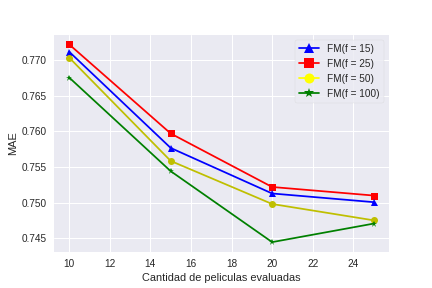
\includegraphics[width=\textwidth]{graficos/entr-factores-mae.png}
            \caption{Errores MAE}
            %\label{fig:SRl2}
    \end{subfigure}
    \caption{Comparación del rendimiento de los modelos de FM con las diferentes cantidad de factores}\label{fig:comp-fact}
\end{figure}

\section{Simulación 3 - Arranque en Frío}

El objetivo de esta simulación es la de analizar el rendimiento de las propuestas realizadas basadas en los vecinos más cercanos para el caso del arranque en frío para un nuevo usuario en la sección \ref{cap:propuestas}, sin recurrir al proceso de encuestas.

\subsubsection{Procedimiento}

Para esta simulación, utilizamos el mismo procedimiento que el utilizado en la simulación de entrevistas, sin la necesidad seleccionar los usuarios para el conjunto de entrenamiento $T$ según la cantidad de ratings. En esta simulación, de un total de 943 usuarios, 786 usuarios pertenecen a $E_{us}$ y 157 usuarios pertenecen a $T_{us}$.

Una vez construidos estos conjuntos, entrenamos nuestra FM, con los parámetros $\alpha$ y $\lambda$ preestablecidos como en la tabla\ref{tb:params1} y calculamos el error en $T$ de la misma manera que lo hicimos en la simulación dos, pero esta vez no necesitamos re-entrenar el modelo, dado que no modificamos nuestros conjuntos. Luego calculamos el promedio de esos errores sobre los usuarios. A esta forma de predecir los ratings, utilizando el vector de variables como fue descrito en \eqref{eq:m1-base}, lo llamamos \textbf{M1}.

En este caso, la FM que consideramos es \textbf{FM-all}, que utiliza todas las variables contextuales. La única salvedad que realizamos fue la de no categorizar la edad, quedando entonces las variables:

\begin{equation*}
x \in \mathcal{B}^{786} \times \mathcal{B}^{1642} \times \mathbb{R}^{25} \times \mathbb{R}^{19} 
\end{equation*}

Para cada usuario $u$, calculamos $N_k(u)$ a los $k$ vecinos más cercanos de $u$. Llamamos \textbf{M-uniforme} a la predicción obtenida al modelar al usuario como \eqref{prop1}, pesando a los vecinos modelo de forma uniforme. \textbf{M-pesado} a la predicción obtenida al modelar el usuario como \eqref{prop2}, donde pesamos a los vecinos por los inversos de las distancias al usuario activo.

\subsubsection{Resultados}

Los resultados obtenidos con la predicción \textbf{M1} fueron:

\begin{equation*}
\text{RMSE} = 1.864,\quad \text{MAE}= 1.125
\end{equation*}

Estos valores los utilizamos para comparar el rendimiento de nuestros modelos de vecinos \textbf{M-uniforme} y \textbf{M-pesado}. 

A continuación, en la figura \ref{fig:cold1} se observan los gráficos de los resultados obtenidos para ambos modelos según la cantidad de vecinos $k$ utilizados y en la figura \ref{fig:cold2} vemos un detalle de los errores en el caso de la predicción según \textbf{M-uniforme}.

\begin{figure}[ht]
\centering
    \begin{subfigure}[b]{0.5\textwidth}            
            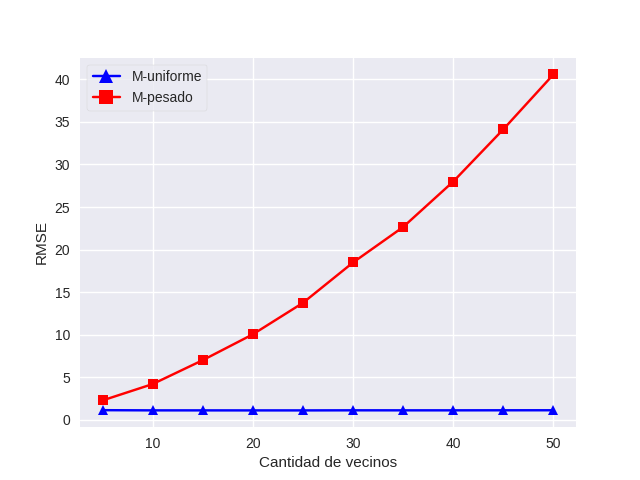
\includegraphics[width=\textwidth]{graficos/cold-1-rmse.png}
            \caption{Errores RMSE}
            %\label{fig:SRl}
    \end{subfigure}%
     %add desired spacing between images, e. g. ~, \quad, \qquad etc.
      %(or a blank line to force the subfigure onto a new line)
    \begin{subfigure}[b]{0.5\textwidth}
            \centering
            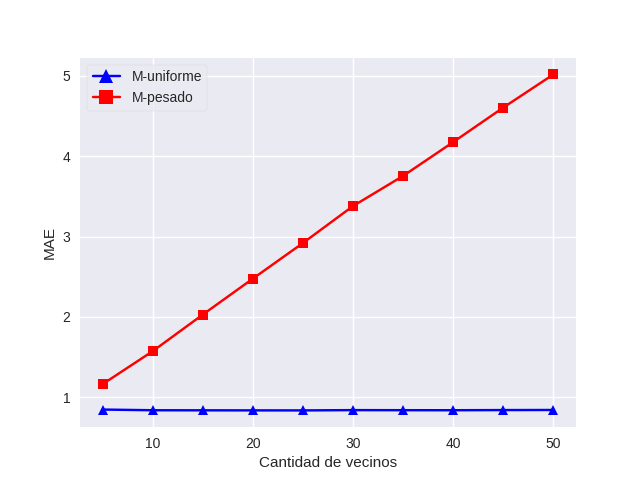
\includegraphics[width=\textwidth]{graficos/cold-1-mae.png}
            \caption{Errores MAE}
            %\label{fig:SRl2}
    \end{subfigure}
    \caption{Errores de \textbf{M-uniforme} y \textbf{M-pesado}}\label{fig:cold1}
\end{figure}

\begin{figure}[!ht]
\centering
    \begin{subfigure}[b]{0.5\textwidth}            
            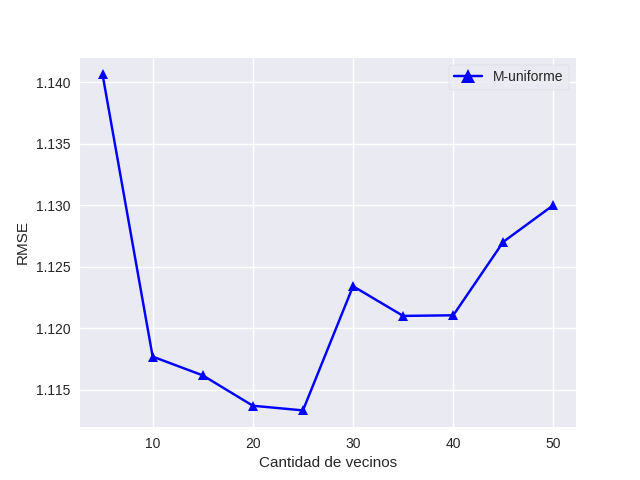
\includegraphics[width=\textwidth]{graficos/cold-2-rmse.png}
            \caption{Error RMSE}
            %\label{fig:SRl}
    \end{subfigure}%
     %add desired spacing between images, e. g. ~, \quad, \qquad etc.
      %(or a blank line to force the subfigure onto a new line)
    \begin{subfigure}[b]{0.5\textwidth}
            \centering
            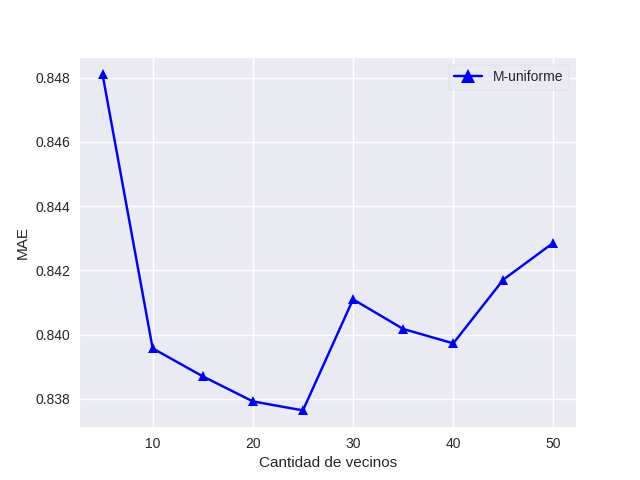
\includegraphics[width=\textwidth]{graficos/cold-2-mae.png}
            \caption{Error MAE}
            %\label{fig:SRl2}
    \end{subfigure}
    \caption{Detalle de los errores de \textbf{M-uniforme}}\label{fig:cold2}
\end{figure}

Los primeros resultados obtenidos muestran que la predicción del modelo \textbf{M-pesado}, obtuvo errores extremadamente altos en ambas métricas y una tendencia clara de aumentar a la hora de considerar más vecinos, lo cual al principio parecería ir en contra de la intuición. No obstante, al observar la forma de modelar al usuario nuevo y estudiar las vecindades de los usuarios que obtuvieron errores de gran magnitud, se pueden determinar algunas causas probables. Al observar en detalle los usuarios que obtuvieron errores de gran magnitud, pudimos ver que estos usuarios, poseían en su mayoría vecinos que se encontraban a distancia cero o a lo sumo uno. Esto provoca que a la hora de realizar la predicción, los términos de $\hat{y}$ que involucran a los factores de los usuarios, queden multiplicados por $\frac{1}{\sqrt{k}}$ en vez de $\frac{1}{k}$. Entonces en estos casos, al multiplicar por $(\sqrt{k})^{-1}$, el modelo no calcula un promedio de los parámetros $w$ y $\textbf{V}$ correspondientes, dando lugar a la aparición de valores extremos en los errores.

Para evitar este problema, proponemos elegir parámetro de contracción al mismo $k$. De esta forma la predicción sobre un usuario $u$, es una combinación entre las dos ideas originales. Si $u$ es el nuevo usuario, lo modelaremos: 

\begin{equation}
\label{prop3}
x_v^{(u,j)}=
\begin{cases}
\frac{1}{d(u,v)+ k} &\text{si } v\in N_k(u) \\
0 &\text{caso contrario}
\end{cases}
\end{equation}

Llamaremos a este modelo \textbf{M-corregido}.


\begin{figure}[ht]
\centering
    \begin{subfigure}[b]{0.5\textwidth}               
		\centering
		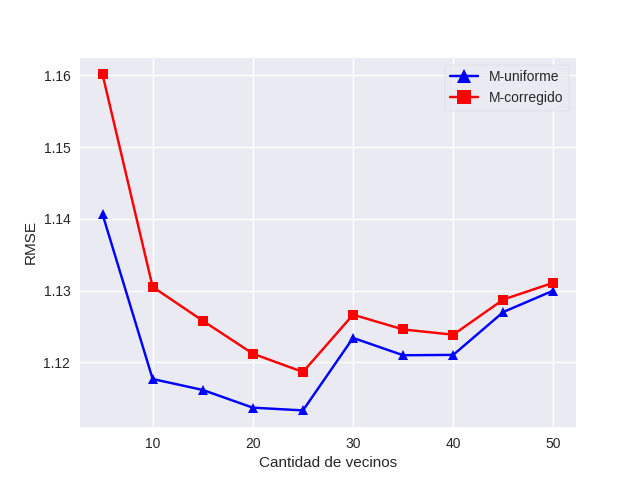
\includegraphics[width=\textwidth]{graficos/cold-3-rmse.png}
		\caption{RMSE}\label{fig:cold3-rmse}
    \end{subfigure}%
     %add desired spacing between images, e. g. ~, \quad, \qquad etc.
      %(or a blank line to force the subfigure onto a new line)
    \begin{subfigure}[b]{0.5\textwidth}
	  \centering
		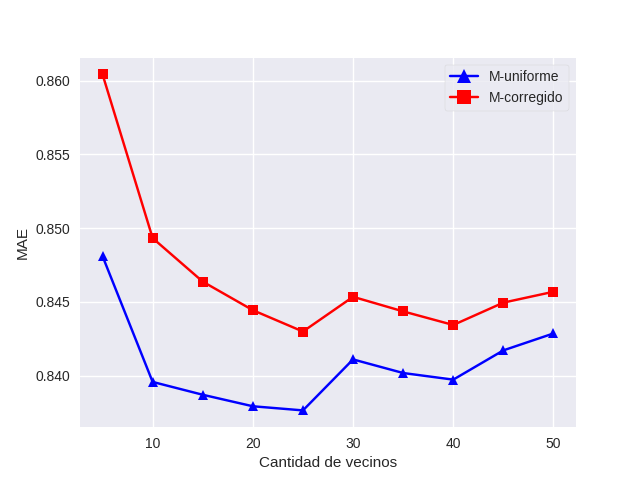
\includegraphics[width=\textwidth]{graficos/cold-3-mae.png}
		\caption{MAE}\label{fig:cold3}
    \end{subfigure}
    \caption{Errores de \textbf{M-uniforme} y \textbf{M-corregido}}\label{fig:cold4}
\end{figure}

En las figuras \ref{fig:cold3-rmse} y \ref{fig:cold3} observamos las comparativas entre \textbf{M-uniforme} y \textbf{M-corregido}, según la cantidad de usuarios considerados como vecindario. En ambos casos se ve que los errores tienen un comportamiento similar. Aumentar la cantidad de vecinos mejora al principio los errores, pero no siempre, ya que luego de considerad 25 vecinos, los errores de ambos empeoran.

El rendimiento de \textbf{M-uniforme} fue superior al rendimiento obtenido por \textbf{M-corregido}. Por lo tanto, esto nos permite inferir que la inclusión de las distancias, a la hora de modelar por utilizando los usuarios vecinos, no ayuda al rendimiento del sistema sobre nuevos usuarios.

\begin{table}[ht]
\centering
\begin{tabular}{|c|c c|}
\hline
Modelo & RMSE & MAE \\
\hline
\textbf{M1} & 1.864398 & 1.125662\\
\textbf{M-uniforme}(k=25) & 1.113308 & 0.837641 \\
\textbf{M-corregido}(k=25)& 1.118658 & 0.842989 \\
\hline
\end{tabular}
\caption{Mejores resultados obtenidos con los modelos propuestos}
\label{tb:resul-prop}
\end{table}

Ambos métodos obtienen su mejor error cuando consideraron 25 vecinos. En este valor, el modelo \textbf{M-uniforme} obtuvo $RMSE = 1.113$ y $MAE=0.837$ , mientras que el modelo \textbf{M-corregido} obtuvo $RMSE = 1.118$ y $MAE = 0.842$. Esto representa una mejora significativa a tratar de predecir los ratings de usuarios nuevos sin realizar ningún tipo de ajuste, como figura en la tabla \ref{tb:resul-base}.

%%%%%%%%%%%%%%%%%%%%%%%%%%%%%%%%%%%%%%%%%%%%%%%%%%%%%%%%%%%%
%%%%%%%%%%%%%%%%%%%%%%%%%%%%%%%%%%%%%%%%%%%%%%%%%%%%%%%%%%%%
\chapter{Conclusiones y Trabajo Futuro}

\section{Escenario clásico}

\subsubsection{Conclusiones}

Considerando los resultados obtenidos, queda claro que las máquinas de factorización poseen un gran potencial en lo que respecta a los sistemas de recomendación, sobretodo en el problema de predicción de ratings, en el cual obtuvo resultados mucho mejores según el error cuadrático medio, mientras que en MAE solo se vio superado por SVD. Que el rendimiento de las máquinas de factorización sea mucho mejor en RMSE que en MAE, era esperable puesto que la función de pérdida considerada es justamente la pérdida cuadrática.

En el caso de recomendación, no obtuvimos tan buenos resultados como para el problema de predicción, ya que a penas se equipara en rendimiento Slope One. Sin embargo, al utilizar como pérdida la función de pérdida cuadrática, es esperable que el rendimiento en la predicción sea mejor que el rendimiento en la recomendación.

\subsubsection{Trabajo Futuro}

La escalabilidad y buen rendimiento de las máquinas de factorización es una de las características que la hace una de las técnicas del estado-del-arte en los sistemas de recomendación. Queda como trabajo futuro, estudiar su comportamiento en conjuntos de mayor tamaño como son el conjunto de datos 26M de MovieLens con 26 millones de ratings de películas\footnote{https://grouplens.org/datasets/movielens/latest/} o el conjunto de 100 millones de ratings de Netflix\footnote{https://www.kaggle.com/netflix-inc/netflix-prize-data/data}.

Por otro lado, considerando los resultados obtenidos en el problema de recomendación, queda como trabajo a fururo la implementación de otras funciones de pérdida objetivo que involucren el ranking de los items y no el rating. Dos de ellas, frecuentemente utilizadas, son la BPR descrita en Rendle et. al.\cite{rendle2009bpr} o WARP, descrita en Weston et. al.\cite{weston2011warp}.

%Queda realizar es una búsqueda exhaustiva de parámetros (tasa de aprendizaje, término de regularización, factores, etc.), ya que utilizamos parámetros preestablecidos para calcular los modelos. Realizar esto podría aumentar significativamente el rendimiento de nuestro sistema pero en un principio, esto sería mas costoso computacionalmente. También es posible un detallado estudio de las variables (ingeniera de variables) lo cual excede el estudio de esta tesis, para ver si alguna de ellas es redundante, o cuales son las más importantes.

Cabe destacar que no utilizamos la información de los códigos postales, es un trabajo a futuro incluirlas en el modelo de máquinas de factorización. Para eso podríamos utilizar los códigos para conseguir variables demográficas como el nivel de educación promedio, el nivel de ingresos promedio, si se trata de una zona urbana o rural, etc.

\section{Escenario arranque en frío}

\subsubsection{Conclusiones}

Los resultados obtenidos en las simulaciones 2 y 3, muestran que las máquinas de factorización realizan predicciones confiables bajo datos ralos, ya que en el caso de entrevistas, tiene. No solo esto, sino que también se pudo observar que la cantidad de factores en el caso del arranque en frío mejoran los resultados, pero que con pocos factores podemos obtener buenos resultados frente a técnicas como SVD.

Por otro lado, nuestra propuesta parece ayudar a mitigar el problema de arranque en frío para un nuevo usuario, reduciendo el error de predicción de ratings al utilizar un modelado del usuario basado en sus características poblaciones con un bajo costo computacional en comparación al modelado por entrevistas. Este escenario, se vería probablemente beneficiado de una ingeniería de variables, ya que al involucrar mayor cantidad de variables y de mejor calidad podremos mejorar la expresividad del modelo.

\subsubsection{Trabajo Futuro}

Como trabajo futuro, quedaría realizar una comparación con las técnicas mas modernas que no utilizan entrevistas, como las descritas en Son\cite{CS:New-son2016dealing}, con nuestro modelo propuesto utilizando las máquinas de factorización.

%\begin{itemize}
%\item Feature Engineering
%\item Agregar K-folds CV
%\item Computar los modelos con diferentes funciones de pérdida
%\item Búsqueda de parámetros
%\end{itemize}


%%%%%%%%%%%%%%%%%%%%%%%%%%%%%%%%%%%%%%%%%%%%%%%%%%%%%%%%%%%%
%%%%%%%%%%%%%%%%% BIBLIOGRAFIA %%%%%%%%%%%%%%%%%%%%%%%%%%%%%
%%%%%%%%%%%%%%%%%%%%%%%%%%%%%%%%%%%%%%%%%%%%%%%%%%%%%%%%%%%%

\bibliographystyle{plainyr}
\bibliography{biblio}

%%%%%%%%%%%%%%%%%%%%%%%%%%

\end{document}
